% (c) 2020 Stefan Antonowicz
% Based off of tex found at https://github.com/ludus-leonis/nipajin
% This file is released under Creative Commons Attribution-NonCommercial-ShareAlike 4.0 International License.
% Please do not apply other licenses one-way.

\renewcommand{\yggArcana}{%
  \mychapter{The Arcana}{arcana}
    \begin{center}
    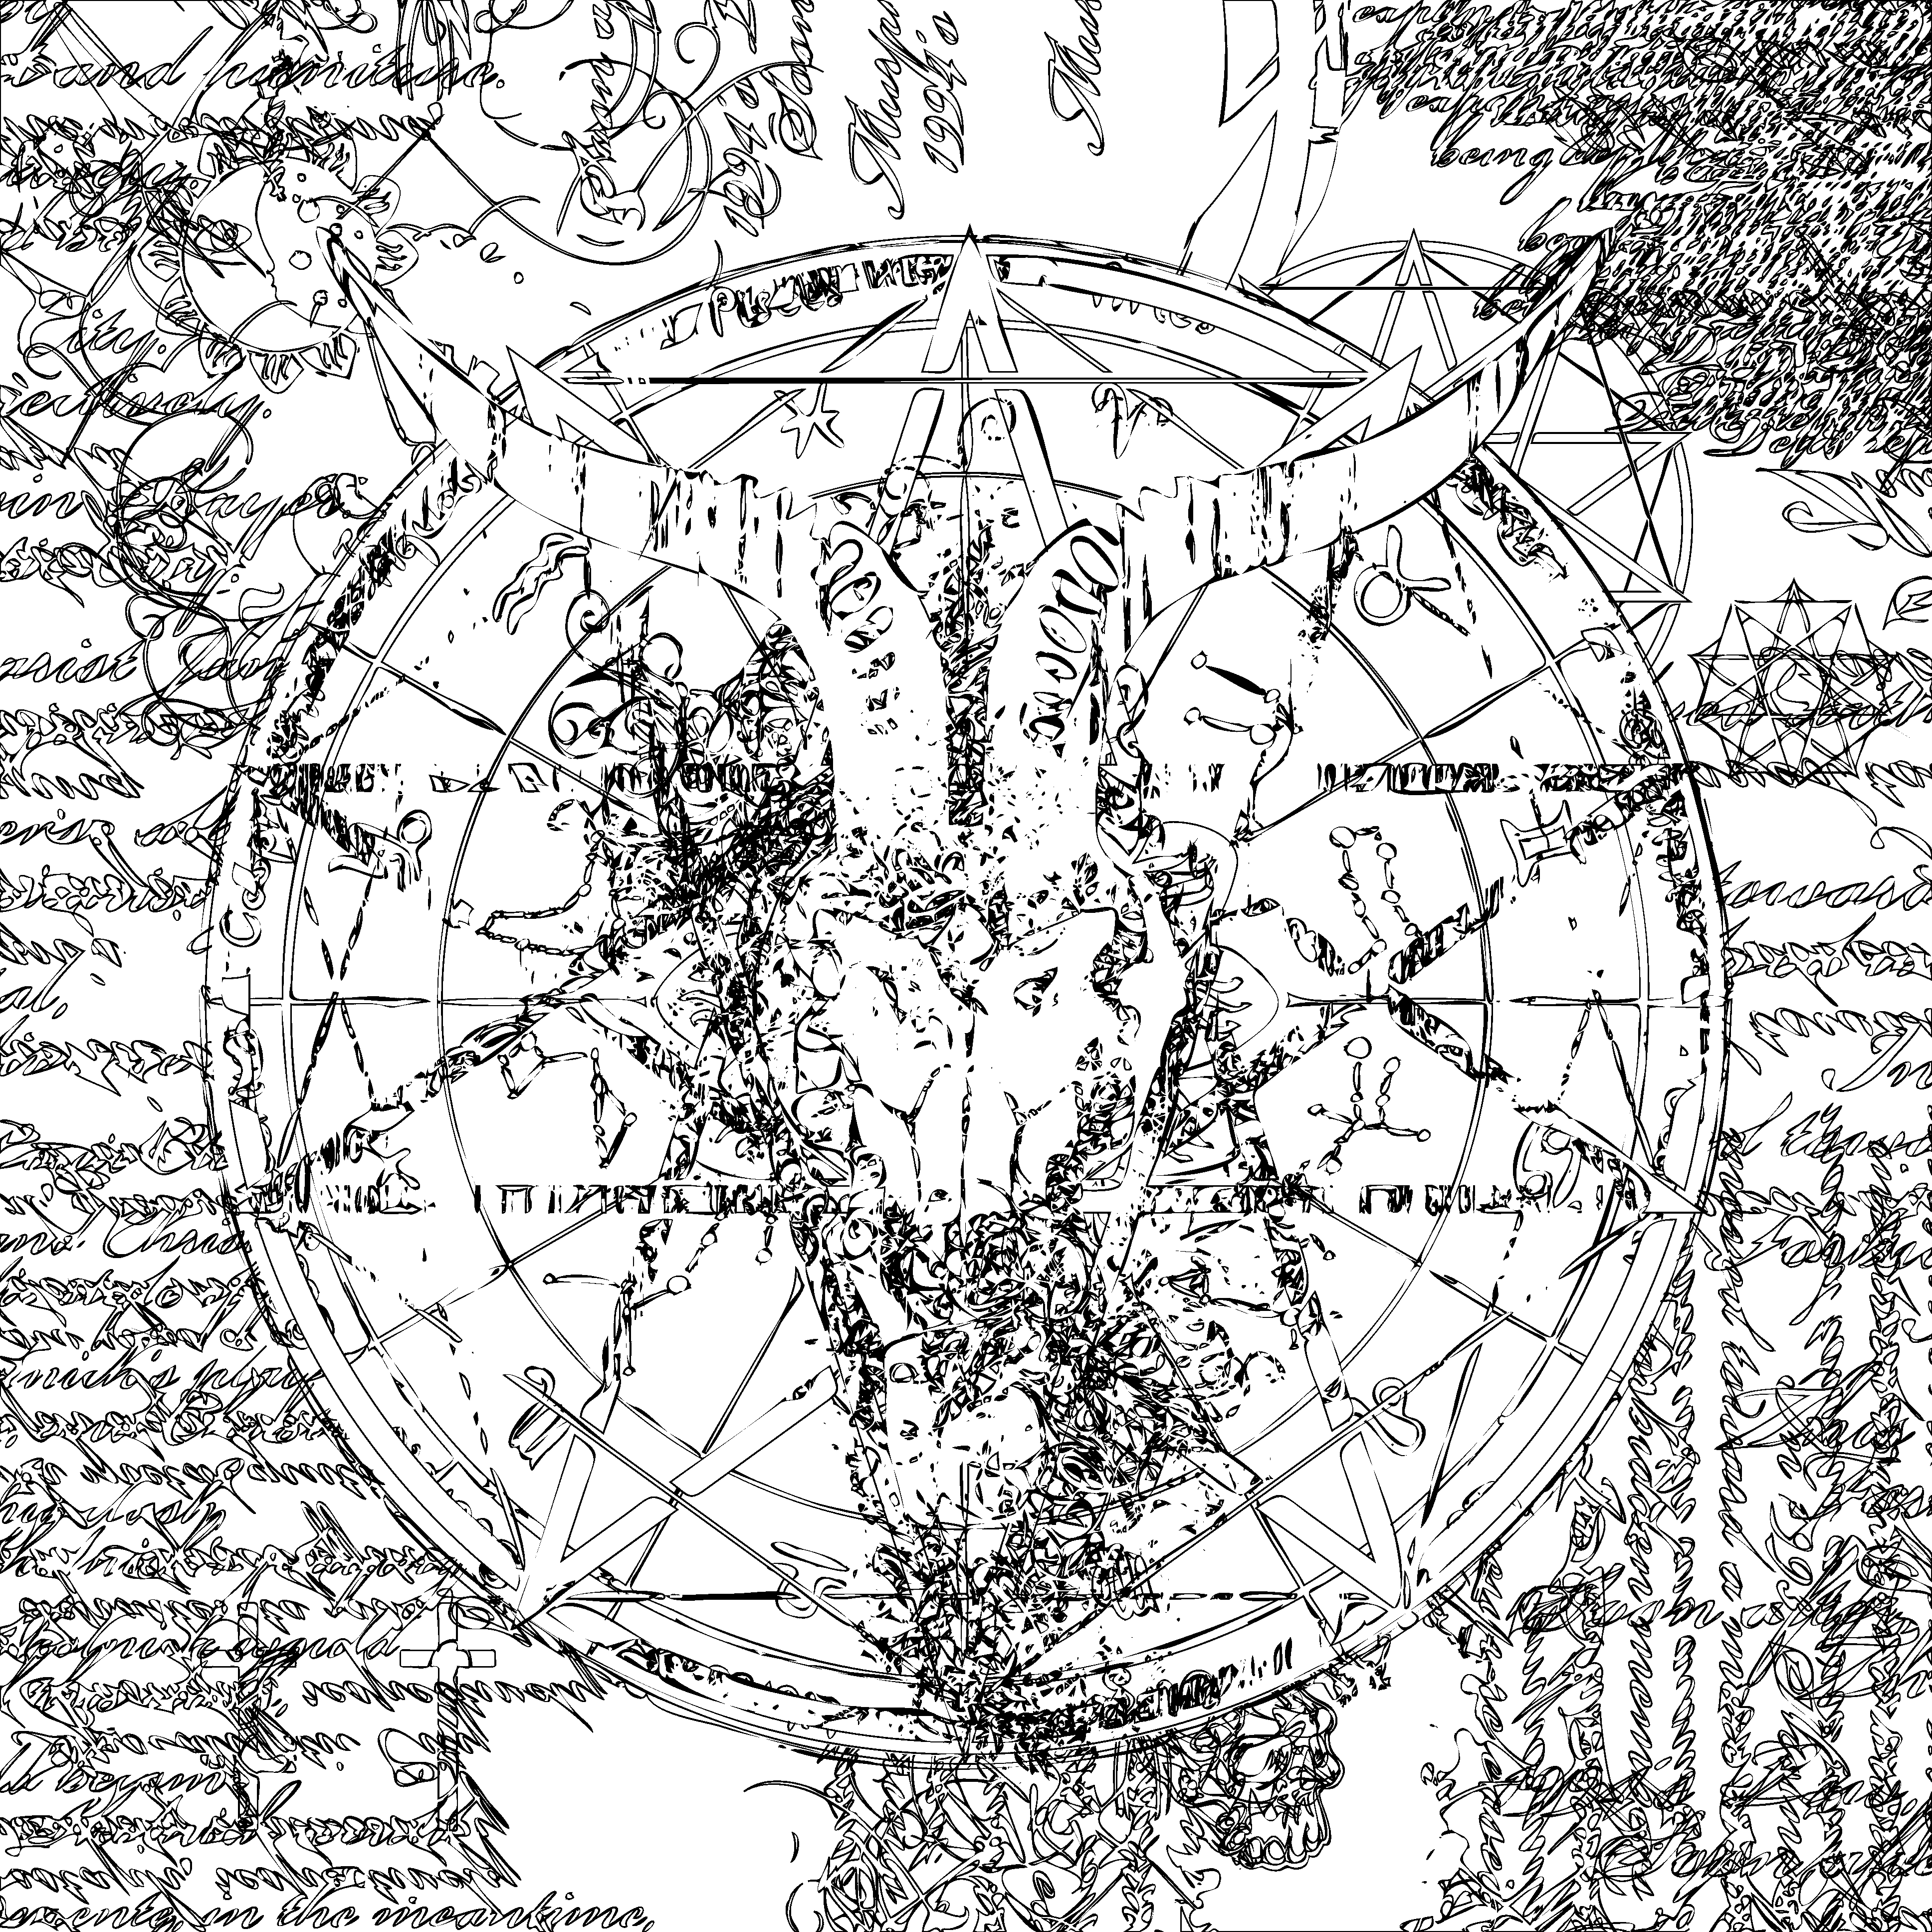
\includegraphics[width=\linewidth,keepaspectratio=true]{arcana/ArcanaHeader}
    \end{center}
    \newpage
}

\renewcommand{\yggArcanaText}{%
\end{multicols*}

Powered by their Crux, the Arcana are the laws, mysteries, chants, balms, scriptures, etc. that manifest the power of \mylink{the Void}{the-void} within \mylink{the Dream}{the-dream}. Each Arcana is associated with one Crux and powered through a Conduit:


\mytable {Y Y Y Y} {
    \thead{Arcana} & \thead{Crux} &  \thead{Conduit} \\
}{
    \mylink{Leechcraft}{arcana-leechcraft} & \mylink{Knowledge}{cruces-knowledge} & \mylink{Ingenuity}{cruces-knowledge-ingenuity} \\
    \mylink{Liturgies}{arcana-liturgies} & \mylink{Faith}{cruces-faith} & \POOLD{d4}  \\
    \mylink{Witchcraft}{arcana-witchcraft} & \mylink{Mojo}{cruces-mojo} & \mylink{Juju}{cruces-mojo-juju}  \\
    \mylink{Wizardry}{arcana-wizardry} and \mylink{Secrets}{arcana-wizardry-secrets} & \mylink{Blood}{cruces-blood} & \POOLD{d6} \\
}

\begin{center}

\mybold{Symbol Key}

\callout {
    \mylist {
      \item \DICE\bgspace The number of dice rolled.
      \item \hrulefill
      \item \SUM\bgspace The sum of the dice rolled.
      \item \hrulefill
      \item \MOD\bgspace A modifier to the roll you make. Can be positive or negative.
      \item \hrulefill
      \item \LENGTH\bgspace How long it takes you to invoke the Arcana. Default is 1 \mylink{Maneuver Action}{combat-maneuvers}.
      \item \hrulefill
      \item \faBullseye\bgspace Who or what you can target, and how far away.
      \item \hrulefill
      \item \faRandom\bgspace If a Secret can be countered by another Secret (and if so, which one).
      \item \hrulefill
      \item \faAnkh\bgspace  The Secret's \mylink{Alignment}{arcana-wizardry-secrets-alignment}.
      \item \hrulefill
      \item \faKey\bgspace Any Keyword(s) associated with the Arcana.
      \item \hrulefill
      \item \faSave[regular]\bgspace Whether or not a victim gets a \SAVE{Hexes} (Yes or No).  The result of a successful Save will be in the Arcana's description.
   }
}

\end{center}

\newpage
\begin{multicols*}{2}


        \newpage

    \mysection{Leechcraft}{arcana-leechcraft}

  \callout {
    Leechcraft uses your \mylink{Ingenuity}{cruces-knowledge-ingenuity}. Unless otherwise noted, Leechcraft takes 2 Actions to perform. You and your patient \mybold{cannot move} while you are applying your medicines.  Leechcraft requires both hands free, but does not require speech. Leechcraft can be performed both on yourself or an Ally (unless indicated otherwise).
}


  \LEECHCRAFT[
    Name=Bedevil Toxin,
    Link=leechcraft-bedevil-toxin
  ]

  Try your \INGENUITY once for a Noxious (d6) Toxin; twice for a Deadly (d10) Toxin; or three times for a Lethal (d16) Toxin. If you don't roll \mybold{any} Failures, you may immediately end a Toxin's effect on your patient. 


  \LEECHCRAFT[
    Name=Bonesetting,
    Link=leechcraft-bonesetting
  ]

  Try your \INGENUITY. If you don't roll a Failure, you may purge a single, non-permanent \mylink{Wound}{physical-wound} (but not a \mylink{Beating}{physical-wound-beating}). Permanent wounds (like missing teeth) can't be fixed with Bonesetting. This Leechcraft can only be performed during a \mylink{Bivouac}{combat-resting-bivouac}.

  \LEECHCRAFT[
    Name=Examination,
    Link=leechcraft-examination
  ]

    Try your \INGENUITY. If you don't roll a Failure, you understand one physical ailment of your patient. This can include: how much health they have left, what disease they're affected by, how many minutes they have left of suffering from a Toxin, and any other physical disorder at the Arbiter's discretion. You must try your \INGENUITY multiple times if you wish to discover more than one ailment. The patient must have an anatomy you roughly understand (again at the Arbiter's discretion).

\cbreak

  \LEECHCRAFT [
    Name=Pharmaceuticals,
    Link=leechcraft-pharmaceuticals
  ]

  Try your \INGENUITY. If you don't roll a Failure, you may purge \mybold{one} of the following effects from an Ally (but not yourself):

\colorcallout{toyeerieblack}{
    \mybullet {
        \item \myital{Adrenal Extract:} \mylink{Stunned}{effect-stunned}
        \item \myital{Blacktoe:} \mylink{Woozy}{effect-woozy}
        \item \myital{Gingeroot:} \mylink{Sickened}{effect-sickened}
        \item \myital{Hair of the Dog:} \mylink{Hung Over}{effect-hung-over}
        \item \myital{Smelling Salts:} \mylink{The Vapors}{effect-the-vapors}
        \item \myital{Trepanation:} \mylink{Concussed}{effect-concussed}
        \item \myital{Woundseal:} \mylink{Bleeding}{effect-bleeding}
    }
}

  \LEECHCRAFT[
    Name=Quarantine,
    Link=leechcraft-quarantine
  ]
  
  Try your \INGENUITY. If you don't roll a Failure, you prevent a person affected by a \mylink{Disease}{vulgate-medicine-diseases} from being contagious for the rest of the Session. Curing the Disease requires \mylink{Medicine}{vulgate-medicine}.

  \LEECHCRAFT[
    Name=Sew Wounds,
    Link=leechcraft-sew-wounds
  ]

  Try your \INGENUITY and heal \SUMDICE Flesh on an Ally (but not yourself) up to their \MAX. This Leechcraft can only be performed during a \mylink{Bivouac}{combat-resting-bivouac}.

  \LEECHCRAFT[
    Name=Stitch,
    Link=leechcraft-stitch
  ]
   
  Try your \INGENUITY on someone who is \mylink{Dying}{combat-dying} (at 0 Flesh). This includes yourself. If you roll a Failure, the patient must immediately make a \DEATH try. Otherwise, they heal 1 point of Flesh (and must immediately make an \INSANITY and \INJURY try). 

\myimage{arcana/PlagueDoctor}

\cbreak

  \LEECHCRAFT[
    Name=Transfusion,
    Link=leechcraft-transfusion
  ]

  Try your \INGENUITY to transfer the blood from one creature to another, including yourself. Both creatures must be alive, in close proximity, and generally immobile during the transfusion. Each Moment, the "donor" loses 1 point of Flesh (or Health), and the "recipient" gains 1 point of Flesh (or Health) up to their \MAX. The Arbiter is under no obligation to tell you how much blood is left in the donor. If the donor is brought to 0 Flesh (or Health) during the transfusion, the recipient must \SAVE{Doom} or fall to 0 Flesh, prompting a roll of their \DEATH. This Leechcraft can only be performed during a \mylink{Bivouac}{combat-resting-bivouac}. 

    \newpage
    % (c) 2020 Stefan Antonowicz
% Based off of tex found at https://github.com/ludus-leonis/nipajin
% This file is released under Creative Commons
% Attribution-NonCommercial-ShareAlike 4.0 International License.
% Please do not apply other licenses one-way.

\end{multicols*}
\mysection{Liturgies}{arcana-liturgies}

The Liturgies are performed using your \mylink{Faith Dice}{cruces-faith}. You must have your \mypg{Holy Symbol}{liturgies-holy-symbol} to perform a Liturgy. Liturgies require both hands and the ability to speak.

When a Liturgy tells you to Spend a Faith Die, roll it and immediately remove it from play. Otherwise, when you try a Faith Die, it is Spent if you roll a Failure (a 1 or a 2). You must declare how many Faith Dice you are committing to invoke a Liturgy before you roll. Details about regaining your Faith can be found in the chapter on the \mypg{Crux of Faith}{cruces-faith}.

\callout {
    There are four formularies of the Liturgies:

    \mybullet {
        \item \mylink{Ablutions}{liturgies-ablutions}: Can only be used on yourself. Take Minutes to perform; cannot be used in Combat.
        \item \mylink{Hymns}{liturgies-hymns}: Can only be used in Combat. Take 1-2 Maneuver Actions to prepare.
        \item \mylink{Lorespells}{liturgies-lorespells}: Can only be used on others. Take Minutes to perform; cannot be used in Combat. 
        \item \mylink{Orisons}{liturgies-orisons}: Can only be used on others in Combat. Take 1 Combat Action to perform.
    }
}


Each Small God shares its Liturgies with the other Small Gods of its \mypg{Paradigm}{faith-paradigm}, though it is possible to find Liturgies that belong to your Small God alone - etched on bronze tablets and hidden by long-dead priests; forgotten in reliquaries lying in pawn shops; or written in the slime of snails tripping balls on 'shrooms.

See the Liturgical Guide in \mypg{Appendix D}{appendix-e} for a list of Liturgies sorted by Paradigm.


\callout{

    For each Liturgy (Novitiates, Clerics, Apostles, and Saints) choose 1 Liturgy aligned with your Paradigm, and 1 of any Paradigm.

\myskip

    Should you take all four Liturgies, you should have 8 Ablutions, Hymns, Lorespells, and/or Orisons in total.
}




\begin{multicols*}{2}



\mysubsection{The Holy Symbol}{liturgies-holy-symbol}

Your Holy Symbol allows you to harness your Faith to perform the Liturgies of your Small God.  Tell the Arbiter what the Holy Symbol of your Small God is (examples of common ones are found in the section on \mylink{the Small Gods}{appendix-d} in Appendix D). Your Holy Symbol is a \mylink{Holy Relic}{miracle-holy-relic}; you must perform the Miracle of \mylink{Holy Relic}{miracle-holy-relic} to create a new one if yours is lost or destroyed.  Remember that your Holy Symbol contains between 1-4 Faith dice that can be counted as part of your pool. If you are separated from your Holy Symbol when you have no Faith pool left (it's stolen or taken from you), or you Spend the Faith that is inside of your Holy Symbol when you have no Faith pool left, you immediately suffer a \mylink{Crisis of Faith}{table-crisis-of-faith}. If the Faith inside of a Holy Symbol becomes completely spent, the Holy Symbol becomes a normal item (and can't be used to perform Liturgies).

Certain Liturgies have a \Duration that depends on the number of Faith \DICE rolled in the invocation:

  \mytable{Y Y} {
    \thead{\DICE}  & \thead{\Duration} \\
  } {
            1 & \DUR{d4} \\
            2 & \DUR{d6} \\
            3 & \DUR{d8} \\
            4 & \DUR{d10} \\
            5 & \DUR{d12} \\
            6+ & \DUR{d16} \\
  }


\newpage

%%%%%%%%%%%%%%%%%%%%%%%%%%%%%%%%%%%%%%%%%%%%%%%%%%%%%%%%%%%%%%%%%%%%%%
%%%%  ABLUTIONS %%%%%%%%%%%%%%%%%%%%%%%%%%%%%%%%%%%%%%%%%%%%%%%%%%%%%%
%%%%%%%%%%%%%%%%%%%%%%%%%%%%%%%%%%%%%%%%%%%%%%%%%%%%%%%%%%%%%%%%%%%%%%



\mysubsection{Ablutions}{liturgies-ablutions}

\callout {
    Ablutions can only be used on yourself; they cannot be invoked on another (though others may gain the benefit of being Close to you). Ablutions take Minutes to perform, and cannot be invoked while in Combat.  Unless stated otherwise, Ablutions vanish at the end of the Session. Each Ablution is distinct and performing it again will remove the previous blessing.
}


\LITURGY [
  Name = Armor of the Gods,
  Link = arcana-mystery-armor-of-the-gods,
  Paradigm = Civilized
]

You summon a suit of holy armor; what the armor looks like is up to you, but it should be elaborate/brutal/gilded etc.\@ (something that makes you stand out in a crowd). You can't wear any other armor while wearing Armor of the Gods.  Your \MD drops to d4; the \UD for the Armor depends on the number of \DICE invested: 1 d4; 2 d6; 3 d8; 4 d10; 5+ d12.  The Armor cannot be repaired; once its \UD is Spent, the Armor disappears.

\LITURGY [
  Name = Barkskin,
  Link = arcana-mystery-barkskin,
  Paradigm = Heathen
]

Spend up to 4 \DICE to become covered in a heavy bark.  Your weight is increased by \DICE x100kg and all physical damage is reduced by -\DICE (minimum 1) - but you can't swim, jump, or run. In addition, you sprout \DICE branches; you may \mypg{Sunder}{combat-deeds-sunder} a branch as if it were a Shield to protect yourself or anyone Close to you from physical damage.


\LITURGY [
  Name = Blessed Brew,
  Link = arcana-mystery-blessed-brew,
  Paradigm = Civilized
]

You create \DICE draughts of a sacramental beer. Each draught grants you +4 Grit (even over \MAX). Any draughts not consumed disappear at the end of the Session.

\LITURGY [
  Name = Children of Shul,
  Link = arcana-mystery-children-of-shul,
  Paradigm = Empyrean
]

You create \DICE small moons that circle the top of your head, casting moonlight Close and Nearby. The shadows thrown by this moonlight give a +\DICE bonus (up to +4) to all \mypg{Whispers}{vulgate-whispers} made by any members of your Band who are Nearby. The moonlight will also activate abilities and powers that manifest in lunar rays (like lycanthropy), and throw light equivalent to \DICE x10 candles.

You can unerringly throw one these moons at Nearby Monsters every Moment, striking for 4 damage each (including creatures only struck by Magic weapons).  When you have no moons left, the liturgy ends. Otherwise the Children of Shul remain for the Session, or until you dispel them.

\LITURGY [
  Name = Corsair's Blade,
  Link = arcana-mystery-corsairs-blade,
  Paradigm = Errant
]

Spend up to 4 \DICE to summon a magical rapier, saber, or cutlass that only you can wield.  The blade is a \FOC weapon that deals \DICE+2 damage. The Corsair's Blade ignores Armor and Soak, and while you wield it you always win Init. The blade is Magic. Because there is no die to roll when dealing damage, it cannot Crit or be Fumbled. The weapon lasts for the Session, or until you dispel it.


\myimage{arcana/Liturgies1}

\newpage

\LITURGY [
  Name = Crusader's Helm,
  Link = arcana-mystery-crusaders-helm,
  Paradigm = Righteous
]


Spend up to 4 \DICE to summon an ivory basinet, complete with crest, neck guard, and visor.  While worn, the Crusader's Helm protects you as a normal helmet (ignore certain Physical Wounds, etc), and you can absorb up to \DICE \mypg{Secrets of the Mind}{arcana-wizardry-secrets-alignment} without effect.  With the visor down you can detect Invisible creatures and are immune to \mylink{The Drop}{combat-drop}. 

\LITURGY [
  Name = Davy Jones's Locker,
  Link = arcana-mystery-davy-joness-locker,
  Paradigm = Cthonic
]

You must be near a body of water to use this liturgy (a river is OK, a puddle isn't).  You summon a chest up to \DICE meters in length, width, and height.  The box can hold up to \DICE X100kg in weight, or about 25 Burden (provided the box is big enough in terms of height, width, and depth i.e. you could lie a 2 meter long pole in a 2 \DICE locker).  Once you seal the box and carve your name onto it, the waters will take the locker back beneath the surface, where it will disappear.  At any time, you can return to the same body of water and bring the locker back from the depths with a word. Otherwise, only your death will return the locker from the deeps, washing up on shore 7 days afterwards for some lucky (or unlucky) soul to find. If you place a living thing inside, it can breathe - but it will starve or die of thirst without food or water (incidentally, this is a great way to make \myital{vodyanoi}).

\LITURGY [
  Name = Doppelg{\UmlautA}nger,
  Link = arcana-mystery-doppelganger,
  Paradigm = Cunning
]

Spend 2 Faith. If you have the opportunity to observe someone for Hours, you can flawlessly disguise yourself as that person - not even their family members will be able to tell the difference at a glance.  While your appearance is identical, you don't have any of their memories or abilities. The Liturgy also grants you the ability to speak any Idiolect or Dialect (if your game uses those rules).

\LITURGY [
  Name = Gory Locks,
  Link = arcana-mystery-gory-locks,
  Paradigm = Monstrous
]

Spend \DICE Faith to turn yourself into a hideous undead caricature of your "normal self".  You immediately gain \effect{Unhallowed} and gain the following effects, based on the number of \DICE spent:  1-2 you are immune to \mypg{Secrets of the Mind}{arcana-wizardry-secrets-alignment}; 3-4 you are immune to \mylink{Toxins}{malignants-toxins}; 5-6 you are immune to \mypg{Secrets of Force}{arcana-wizardry-secrets-alignment}; 7+  you are immune to iron weapons.  These effects are cumulative.

You can only speak Graveborn for the duration of the liturgy.  Your undead form prompts an \INSANITY try or morale check among all who see you (Allies and Monsters alike), unless they have seen you in your undead form before. The liturgy lasts for the Session, or until you dispel it. 

\LITURGY [
  Name = Hand of Fate,
  Link = arcana-mystery-hand-of-fate,
  Paradigm = Ruinous
]

Spend 2 Faith. At any time during the rest of the Session, you may change the face of any die that hits the table (for example, if an Ally were to roll a 1 on a critical roll, you could change it to be a "natural 20"; conversely, you could change a 20 to a "natural 1"). Hand of Fate can only be invoked once per Session. 

\LITURGY [
  Name = Incinerate,
  Link = arcana-mystery-incinerate,
  Paradigm = J{\UmlautO}tnar
]

This liturgy requires you to create a bonfire.  You can place up to \DICE inorganic objects into the fire weighing no more than \SUMDICE kg.  The objects are burned to a pile of enchanted ash, which can be harvested and stored as an insignificant item (0 Burden).  When you wish the objects to become whole again, you must build a fire and sprinkle the ash inside of it; you can reach into the fire unharmed to pull the objects from the flames as they were when you placed them into the fire.  If you perish before the objects are retrieved, the ash reverts to normal, unenchanted ash and the objects are destroyed.


\LITURGY [
  Name = Lady Luck,
  Link = arcana-lady-luck,
  Paradigm = Errant
]

Spend \DICE Faith, but put them to the side instead of removing them from play. For the remainder of the Session, you may roll \mybold{one} of these dice to modify \myital{any} \RO or \RB roll (by Ally or Monster alike) either plus or minus the \SUMDICE of the die roll.  You can only use 1 die per roll.  Regardless of the \SUMDICE of the die, the Faith die is lost the moment it is rolled.  Any unused \DICE are lost at the end of the Session, or if you (re)invoke Lady Luck.


\LITURGY [
  Name = Mirror Image,
  Link = arcana-mystery-mirror-image,
  Paradigm = Cunning
]


You create \DICE illusory images of yourself, which move as you move and always stay Close to you. They are constantly stepping through each other, so that it is impossible to tell which of these is an illusion, and which is the real you. When an enemy attacks you, roll to see if they hit you or an image (equal chance). An image vanishes as soon as it suffers a solid impact (a blow from a mace, but also a slap). Area effects such as a dragon's breath will cause all images to instantly vanish (and you'll take fire breath damage, naturally). The Mirror Images otherwise last until the end of the Session.


\LITURGY [
  Name = Preserve,
  Link = arcana-mystery-preserve,
  Paradigm = J{\UmlautO}tnar
]

By touching an object, you are able to freeze it for a period of time in order to preserve it.  If the object is an Ally or Monster, they must be lying completely still.  Unwilling creatures get a Save.  While frozen, any toxins, diseases, bleeding, or negative effects are stopped for a period of time, depending on the number of dice spent.  You cannot end this liturgy willingly once it has begun, though it could be ended prematurely by great heat (a very large bonfire, for example) or by taking more than \SUMDICE points of damage, which will cause the object to shatter into many pieces.  

1 Faith: Minutes; 2-3 \DICE: Days; 4-5 \DICE: Weeks; 4 \DICE: Months; 6-7 \DICE: Years; 8+ \DICE: Permanent. 


\LITURGY [
  Name = Revered Aegis,
  Link = arcana-mystery-revered-aegis,
  Paradigm = Righteous
]

Spend \DICE Faith. You summon a brightly mirrored shield that can be \mylink{Sundered}{combat-deeds-sunder} up to \DICE times before it disappears.  The shield floats nearby, leaving both of your hands free.  In addition, the mirror of the shield reflects images back in a flattering on unflattering way, depending on your desire, and can be used to reflect / refract light. 

\myimage{arcana/Liturgies2}

\LITURGY [
  Name = Sanguine Remedy,
  Link = arcana-mystery-sanguine-remedy,
  Paradigm = Cthonic
]

You can heal Flesh by drinking another sentient creature's blood.  The creature must be alive when you feast on them; the act of drinking their blood takes their life (kills them).  Spend 1 Faith to Heal yourself to full Flesh and Grit, and make an \INSANITY try.

\newpage

\LITURGY [
  Name = Sacred Smoke,
  Link = arcana-mystery-sacred-smoke,
  Paradigm = Heathen
]

Choose up to \DICE \mylink{Narcotics}{gear-narcotics}, and have your Small God inject them directly into your brain through the Sacred Smoke. Roll \mylink{Addiction}{gear-narcotics-addiction} as normal. This Ablution requires a pipe, but you otherwise don't need to have the drugs in your possession.  See the appropriate sections under \mylink{Gear}{gear} for a list of Narcotics and details on Addiction.

\LITURGY [
  Name = Sceptre of Ruin,
  Link = arcana-mystery-lucky-day,
  Paradigm = Ruinous
]

Spend up to 6 \DICE. A sceptre appears in your hand, glowing with malevolent fire. The sceptre is a 2h \FOC weapon that deals \DICE+\DICE damage. Every time the sceptre deals damage, reduce its damage by 1. The sceptre can strike creatures who are only struck by magical weapons, but because there is no die to roll when dealing damage, it cannot Crit or be Fumbled. 

Once the damage is exhausted (reaches 0), the Sceptre disappears.


\LITURGY [
  Name = Slimeform,
  Link = arcana-mystery-slimeform,
  Paradigm = Monstrous
]

You transform yourself and all of your Gear into a slime.  You can absorb up to \SUMDICE+\DICE damage without any ill effects (damage after this goes straight to Flesh, and immediately ends the liturgy).  You are unable to attack, talk, cast spells, etc while in Slimeform, but you can move at a the pace of a slow walk, climb walls, hang from the ceiling, and slip under the cracks of doors if you wish.  The effect lasts for the Session or until you dispel it.


\LITURGY [
  Name = Welkin's Gaze,
  Link = arcana-mystery-welkin-gaze,
  Paradigm = Empyrean
]

You cast your gaze to the heavens, which will show you events transpiring within \DICE x 50km from you. You only need to describe what you want to see and it will appear, but the vision is misty and it's hard to make out details.  You can't see things that are not exposed to the sky, so if you wanted to "see the body of Sir Tremalane on the northern battlefield", it may only show you the spot where he was buried.


%%%%%%%%%%%%%%%%%%%%%%%%%%%%%%%%%%%%%%%%%%%%%%%%%%%%%%%%%%%%%%%%%%%%%%
%%%%  HYMNS %%%%%%%%%%%%%%%%%%%%%%%%%%%%%%%%%%%%%%%%%%%%%%%%%%%%%%
%%%%%%%%%%%%%%%%%%%%%%%%%%%%%%%%%%%%%%%%%%%%%%%%%%%%%%%%%%%%%%%%%%%%%%

\mysubsection{Hymns}{liturgies-hymns}

\callout {
    Hymns can only be used in Combat. A Hymn will take 1 or 2 Maneuver Actions to prepare i.e. if a Hymn says it takes \myital{1 Maneuver Action}, it will take you 1 Maneuver Action to prepare, and can be used on your second Action. Any effects of Hymns immediately cease at the end of Combat. Unless otherwise noted, if a Hymn is performed again it replaces the previous version of the same Hymn.
}

\LITURGY [
  Name = Abyssal Trident,
  Link = arcana-mystery-abyssal-trident,
  Paradigm = Cthonic,
  Duration=1 Maneuver Action
]

You summon an ethereal trident to your hand. The Abyssal Trident cannot be used in melee, it must be thrown at a Nearby or Far-Away target. The Abyssal Trident is a \FOC weapon that deals \DICE x2 damage. The Abyssal Trident immediately dissipates after it is thrown, or at the end of Combat. 

\LITURGY [
    Name=Blessed Blade,
    Link= arcana-mystery-blessed-blade,
    Paradigm = Righteous,
    Duration=1 Maneuver Action
]

Spend 1 Faith. The weapon you are holding is Magical and cannot be dropped.

\LITURGY [
  Name = Eye of Flame,
  Link = arcana-mystery-eye-of-flame,
  Paradigm = Righteous,
  Duration=1 Maneuver Action
]

Spend 1 Faith. Your eyes burn like coals, allowing you to see all Invisible and hidden things. Knaves who are using the \mylink{Whisper of the Bride}{vulgate-whisper-the-bride} must make a new \mypg{Whisper Try}{vulgate-whispers} against a Target Number of 7. You can also see through darkness (including magical darkness), and are immune to \effect{Blindness}. If you use this while already Blinded, the effect immediately ends.




\LITURGY [
  Name = Great Strength,
  Link = arcana-mystery-great-strength,
  Paradigm = Errant,
  Duration=1 Maneuver Action
]

Spend \myital{1 Maneuver Action} and roll 1 Faith Die. You may add the result of this die to any \RO or \RB try you make that uses \VIG (including using \VIG weapons). You can roll multiple times, but each roll you make takes 1 Maneuver Action. If you do not use add the \SUMDICE to an \RO or \RB try before Combat is over, the bonus is lost.

\LITURGY [
  Name = Hecate's Blessing,
  Link = arcana-mystery-hecates-blessing,
  Paradigm = Cunning,
  Duration=1 Maneuver Action
]

Spend 1 Faith. Until the end of Combat, you may use your Faith to cast \mypg{Wizardry Arcana}{arcana-wizardry} from a \mypg{Fetish}{fetishes}.

\LITURGY [
  Name = Hone,
  Link = arcana-mystery-hone,
  Paradigm = Civilized,
  Duration=1 Maneuver Action
]

You run your finger over your weapon, imbuing it with sacred power. If the object is a Bashing weapon, it deals +\DICE damage; if the object is a Stabbing or Chopping weapon, it deals +\DICE X2 damage. The edge must be smaller than your outstretched arms.


\LITURGY [
  Name = Indomitable Mail,
  Link = arcana-mystery-instantaneous-repair,
  Paradigm = Civilized,
  Duration=1 Maneuver Action
]

Spend 1 Faith. You may repair a suit of Armor up to its \MAX value.

\cbreak

\myimage{arcana/Mystic_2}

\newpage

\LITURGY [
  Name = Lucky Throw,
  Link = arcana-mystery-lucky-throw,
  Paradigm = Ruinous,
  Duration=1 Maneuver Action
]

 You must be holding a Throw weapon. Spend 1 Faith.  You may hurl this weapon up to Far-Away without missing. You do not need to see the Monster, but you do need to know their approximate location, and there must be a clear path you could trace to reach them. The path can be as convoluted as required, bouncing off of walls and ricocheting off the floor. The weapon will pass through any gaps it could reasonably fit through (a hand axe could pass through a crack in a door but not a keyhole, for example).


\LITURGY [
  Name = Misericorde,
  Link = arcana-mystery-misericorde,
  Paradigm = Cthonic,
  Duration=1 Maneuver Action
]

You must be holding an \mybold{iron} Dagger. Spend 1 Faith.  The next time you strike a Monster Close to you with this weapon, it will ignore any Armor, deal \MAX damage, and the victim must Save or be inflicted with \effect{Bleeding}.

\LITURGY [
  Name = Monstrous Aspect,
  Link = arcana-mystery-monstrous-aspect,
  Paradigm = Monstrous,
  Duration=\DICE Maneuvers
]

Gain \DICE of the following \mypg{Monster Traits}{monster-traits}: \mylink{Acidic}{monster-trait-acidic}; \mylink{Amphibious}{monster-trait-amphibious};
\mylink{Cannibal}{monster-trait-cannibal} (taking this Trait requires an \INSANITY try); \mylink{Leaping}{monster-trait-leaping};
\mylink{Pack}{monster-trait-pack} (treat other Adventurers Close to you as "Pack Monsters"); \mylink{Slippery}{monster-trait-slippery} 
\\~ \myital{\DICE Maneuver Actions}


\begin{center}

\includegraphics{arcana/Liturgies4}
\end{center}


\LITURGY [
  Name = Mountainhands,
  Link = arcana-mystery-mountainhands,
  Paradigm = Empyrean,
  Duration=2 Maneuver Actions
]

Your hands enlarge and become stone.  Unarmed Attacks do +\DICE damage (up to a maximum of +4).  In addition, you can reach your hands into substances that might affect Flesh but not stone (fire, boiling water - OK.  Lava or acid - not OK). Your hands must be empty (including rings and gloves) to invoke this Liturgy. This liturgy can only affect two of your arms i.e. it can't be combined with liturgies or spells that give you extra arms.


\LITURGY [
    Name = Pummeling Hands,
    Link = arcana-mystery-pummeling-hands,
    Paradigm = Monstrous,
    Duration=\DICE Maneuvers
]

For every Faith you Spend, an extra arm sprouts from your torso. The arms can hold things for you, and grant you a +4 on any rolls where extra arms might be useful (climbing, swimming, etc.). Wearing armor is impossible when using this Liturgy.

The arms cannot fight with weapons, but you may fight Unarmed with these extra arms (including the \mypg{Grapple Combat Maneuver}{combat-deeds-grapple} ). Treat each arm as a \FOC weapon that deals \DICE damage when it hits. Each attack must be rolled separately.  You cannot Spend more than 6 Faith when invoking this liturgy.


\LITURGY [
  Name = Rending Strike,
  Link = arcana-mystery-rending-strike,
  Paradigm = Ruinous,
  Duration=1 Maneuver Action
]

You must be holding a \mylink{Chopping}{gear-weapons} weapon. Spend 1 Faith. For the rest of Combat, any time the weapon deals damage, the victim must roll their Armor \UD two times.

\newpage


\LITURGY [
  Name = Rootshield,
  Link = arcana-mystery-rootshield,
  Paradigm = Heathen,
  Duration=2 Maneuver Actions
]

Your Faith manifests the very roots of Ygg to defend you. Treat the Rootshield as a \mylink{Shield}{gear-armor} that can be sundered up to \DICE times.

\LITURGY [
  Name = Sirocco,
  Link = arcana-mystery-sirocco,
  Paradigm = Empyrean,
  Duration=1 Maneuver Action
]

Roll 1 Faith. You may add the result of this die to any \RO or \RB try you make that uses \DEX (including using \DEX weapons). You can roll multiple times, but each roll you make takes 1 Maneuver Action. If you do not use add the \SUMDICE to an \RO or \RB try before Combat is over, the bonus is lost.

\LITURGY [
  Name = Trollblood,
  Link = arcana-mystery-trollblood,
  Paradigm = J{\UmlautO}tnar,
  Duration=2 Maneuver Actions
]

Spend up to 4 Faith. As long as you are not Dying, you regenerate +\DICE Flesh at the bottom of each Moment. If you ever it 0 Flesh and begin Dying, this Liturgy immediately ends. The regeneration is negated if the damage is from an acid or fire source. At the end of Combat, this liturgy immediately ends (before you can take a Breather).


\LITURGY [
  Name = Vaulting Step,
  Link = arcana-mystery-vaulting-step,
  Paradigm = Errant,
  Duration=1 Maneuver Action
]

Your next \DICE+\DICE strides (about 1m each stride) land on a plane of Force the size of your foot.  The step can be taken in any direction up, down, sideways, or across (though you cannot pass through physical objects).  You can combine these in any way you want - stride 45 degrees into the air, take another step up, and a final step down (for example).  Your final step must be on a solid surface, or you fall.

\LITURGY [
  Name = Vulpine Wisdom,
  Link = arcana-mystery-vulpine-wisdom,
  Paradigm = Cunning,
  Duration=1 Maneuver Action
]

Roll 1 Faith. You may add the result of this die to any \RO or \RB try you make that uses \INT (including using \INT weapons). You can roll multiple times, but each roll you make takes 1 Maneuver Action. If you do not use add the \SUMDICE to an \RO or \RB try before Combat is over, the bonus is lost.

\myimage{arcana/Liturgies5}

\LITURGY [
  Name = Whip of Thorns,
  Link = arcana-mystery-whip-of-thorns,
  Paradigm = Heathen,
  Duration=1 Maneuver Action
]

A veridian scourge appears in your hand, studded with thorns. The Whip of Thorns is a \FOC Brawl weapon that deals \DICE damage. If the Whip strikes Flesh, the victim must Save or be inflicted with the \effect{Bleeding}.

\LITURGY [
  Name = Witness Me,
  Link = arcana-mystery-witness-me,
  Paradigm = J{\UmlautO}tnar,
  Duration=1 Maneuver Action
]

Gain +\DICE on your Attack tries, and deal +\DICE damage if your try succeeds.  At the end of Combat, you immediately catch \effect{the Vapors}, drop to 0 Flesh, and must immediately make a \DEATH try.



\newpage

%%%%%%%%%%%%%%%%%%%%%%%%%%%%%%%%%%%%%%%%%%%%%%%%%%%%%%%%%%%%%%%%%%%%%%
%%%%  LORESPELLS %%%%%%%%%%%%%%%%%%%%%%%%%%%%%%%%%%%%%%%%%%%%%%%%%%%%%%
%%%%%%%%%%%%%%%%%%%%%%%%%%%%%%%%%%%%%%%%%%%%%%%%%%%%%%%%%%%%%%%%%%%%%%

\mysubsection{Lorespells}{liturgies-lorespells}
\callout {
    Incantations of utility and assistance. Lorespells take Minutes to perform, and cannot be used in Combat. Unless otherwise noted, you cannot target yourself with a Lorespell. Each Lorespell is distinct; if a Lorespell is performed again, it replaces the previous version of the same Lorespell.
}

\LITURGY [
  Name = Army of the Pharaohs,
  Link = arcana-mystery-army-pharaohs,
  Paradigm = Civilized,
  Duration = Session
]

Spectral workmen spring into being, ready to do your bidding. They can only perform one of these tasks per invocation of the Lorespell (but it can be invoked multiple times):

\callout{\footnotesize{
\mybullet {
    \item If the spirits have access to a forge, they can create \DICE x 1000 spears and shields (any combination) out of earth and stone. The armaments disappear at sunset unless the Lorespell is reinvoked.
    \item The spirits will fell a tree no larger than \DICE X 5m tall and \DICE meters in diameter. Depending on the number of \DICE, the felled tree is: 1) cut and broadly de-limbed; 2) cut, de-limbed, and debarked; 3) cut, de-limbed, debarked, cut into planks as per your specifications, and stacked; 4) cut, planed, de-limbed, debarked, cut into planks, stacked, sanded, and finished.
    \item The spirits clear \DICE x 7m of earth from a trench. You may divvy these \DICE up among length, width, and height as you wish (for instance, a 1 \DICE trench might be 5m x 1m x 1m, or 3m x 2m x 2m, etc).
    \item The spirits bless up \DICE Flasks of Oil, Personal Provisions, Quivers of Arrows/Bolts, Torches, or Narcotics. For the rest of the Session, these blessed items do not need to roll their \UD when utilized. See the sections on \mylink{Tools of the Trade}{gear-equipment} and \mylink{Narcotics}{gear-narcotics} under \mypg{Gear}{gear} for more details.
}}}

\cbreak

\LITURGY [
  Name = Capture Wind,
  Link = arcana-mystery-capture-wind,
  Paradigm = Errant,
  Duration = Session
]

A circle \DICE meters in radius extends from your fingertips in front of you. As long as you maintain \mylink{Concentration}{time-concentration}, you can absorb any wind passing through the circle. 

The wind is stored inside of the circle, similar to \mylink{Hammerspace}{meta-hammerspace}. At any time during the Session, you can reactivate the circle to release the wind you absorbed.  The wind flows out at the same rate it entered. If you activate this Lorespell in a light breeze for 5 minutes, it will release a light breeze over 5 minutes. The wind only flows from the circle, so anyone standing behind it is not affected (unless you release hurricane-force winds indoors). 

The circle disappears (taking the wind with it) at your command, if you ever go to 0 Flesh, or at the end of the Session.

\LITURGY [
  Name = Clearwater,
  Link = arcana-mystery-clearwater,
  Paradigm = Heathen,
  Duration = Session
]

You create \DICE draughts of cold, clear water. When drunk by Mortals, the Clearwater restores +4 Grit (even above \MAX). When drunk by Unseelie, treat as a \mylink{Noxious (d6)}{malignants-toxins} Toxin. The draughts must be drunk before the end of the Session, or they revert to regular (though very clean) water. You are unable to drink Clearwater you have created.

\LITURGY [
  Name = Dirge,
  Link = arcana-mystery-dirge,
  Paradigm = J{\UmlautO}tnar,
  Duration = Session
]

Up to \DICE Allies who have died (failed their \mylink{Death try}{combat-dying}) can attempt one final Death try. The Ally must have died this Session and their corpse must be Close by. If the Ally should roll and survive, it turns out they were just "mostly dead" - they return with 1 Flesh, and must make an immediate \mylink{Injury}{adventurer-kismet-injury} try. The Ally must also immediately roll on the \mypg{Greater Curse}{table-greater-curses} table (cheating death has its costs). The Dirge won't help anyone with an ... extreme ... death (burned to a crisp, beheaded, etc.) at the Arbiter's discretion.



\LITURGY [
  Name = Fortifying Blaze,
  Link = arcana-mystery-fortifying-blaze,
  Paradigm = Righteous,
  Duration = Bivouac
]

Up to \DICE Allies (but not yourself) can step into the flames of a Fortifying Blaze. The Ally immediately takes 1 damage to Flesh but no further damage. They must remain in the Fortifying Blaze for Minutes to gain any benefit; during this time they cannot lie, and must answer truthfully any question asked of them.  After the duration has expired, they may choose one of the following benefits for the remainder of the Session:

\callout{\footnotesize{
\mynumlist {
    \item Gain +2 to any damage rolls;
    \item Gain +4 to all Saves;
    \item Gain +4 on all Skill tries;
    \item Only fail a \DEATH try on a 1 (instead of a 1 or 2);
    \item Only fail an \INSANITY try on a 1 (instead of a 1 or 2);
    \item Only fail an \INJURY try on a 1 (instead of a 1 or 2).
}}}

Fortifying Blaze requires a campfire, and cannot be used at the same time as \mylink{Hearthfire}{arcana-mystery-hearthfire}.


\LITURGY [
  Name = Giantform,
  Link = arcana-mystery-giantform,
  Paradigm = J{\UmlautO}tnar,
  Duration = Session
]

A bipedal Ally or Monster who is Close or Nearby to you grows \DICE x 500cm in height, with strength to match. Unarmed Attacks do an extra point of damage for every 2 \DICE you spend, and the target can lift an additional \DICE x100kg. If the creature is wearing Armor when Giantform is invoked, the creature must immediately roll that Armor's \UD. The creature must take the result in damage to Flesh, and the armor is ruined (drops to 0 \MAX \UD).  "Normal" sized weapons are unusable in Giantform. The Giantform lasts for the Session, or until you dispel it.

\LITURGY [
  Name = Hearthfire,
  Link = arcana-mystery-hearthfire,
  Paradigm = Heathen,
  Duration = Bivouac
]

During a \mylink{Bivouac}{combat-resting}, you imbue your campfire with healing properties. The Hearthfire will prevent any \mylink{Wandering Monsters}{arbiter-monsters-wandering} from attacking your camp. Up to \DICE Allies (but not yourself) may gain up to \DICE benefits; each person can pick their own benefit, but they can only pick each benefit once.  The healing is \mybold{in addition} to the effect of taking the Bivouac as normal.

\callout{\footnotesize{
\mybullet {
    \item Restore 1 Flesh.
    \item Restore 1 \UD of your \mylink{Armor}{gear-armor}, up to its \MAX.
    \item Restore \DCUP of any \myital{one} aspect of your \mylink{Personality}{adventurer-personality}.
    \item Restore \DCUP of your \mylink{Prowess}{sellsword-prowess}.
    \item Restore \DCUP of your Lucky Die (\mylink{Knave}{knave-lucky-die} or \mylink{Pooka}{pooka-lucky-die}).
    \item Restore \DCUP of your \mylink{Juju}{cruces-mojo-juju}.
    \item Restore \DCUP of your \mylink{Ingenuity}{cruces-knowledge-ingenuity}.
    \item Restore 2 \mylink{Blood Dice}{cruces-blood-dice}.
    \item Restore your \mylink{Grace Die}{vulgate-sacraments-grace}.
}}}

Note that "up to \MAX" is implied in all of the above. Hearthfire requires a campfire, and cannot be used at the same time as \mylink{Fortifying Blaze}{arcana-mystery-fortifying-blaze}.

\LITURGY [
  Name = Lay Assistance,
  Link = arcana-mystery-lay-assistance,
  Paradigm = Civilized,
  Duration = See Below
]

Choose one of the following effects:

\mybold{Banker:}  Convert up to \SUMDICE kg of coins into coins of another type of equivalent value (reminder that there are 100 coins in a kg, and 4 kg of coins are 1 Burden). For example, if the \SUMDICE of your dice roll was 10 you could convert 1,000 iron pieces (10kg) into 100 silver pieces (1kg) or 10 gold pieces (1/10kg); or you could convert 10 gold pieces into 100 silver pieces or 1,000 iron pieces. 

\mybold{Collector of Alms:} During the \mylink{Shopping Step}{downtime-shopping} of \mylink{Downtime}{downtime}, you can convert Faith directly into coin.  Roll \DICE Faith.  For every 2 you get, gain 50\FE (and lose the die); for every 3 you get, gain 10\AG; for every 4 you get, gain 2\AU. Any unused money disappears at the end of the \mylink{Shopping Step}{downtime-shopping}

\mybold{Exchequer:} Place up to \DICE X100kg of coins into \mylink{Hammerspace}{meta-hammerspace} for an indefinite period of time; the coins essentially cease to exist, have no Burden, and cannot be stolen or taken by others (though the existence of the coins can be divined through \mylink{Scrying}{occultism-descry}).  You can retrieve the coins at any time (though you have to retrieve all of them at once).  The coins are also released upon your death, meaning that you might occasionally be a target of thieves. You can combine the effects above (so you could convert money and store it in Hammerspace if you'd like).  You must invoke this liturgy each time you want to put more coins into Hammerspace, but everything that's in Hammerspace is released either when you will it, or upon your death.

\mybold{Stevedore:} Up to \DICE X250kg of nonliving objects, as you designate, are packed neatly. You must name the objects or their general category when you invoke this liturgy ("those coins", "the contents of that room") If no packing materials are provided, the objects will be stacked into compact cubes, with the largest and most stable objects at the bottom. If chests, paper and twine, sacks, carts, etc. are provided, the are used as you direct. The packages created will take up the minimum space possible, and will be remarkably sturdy. Objects will continue to be packed as long as you maintain \mylink{Concentration}{time-concentration}. The objects must be able to move freely (you wouldn't be able to pack the clothes someone was wearing, for instance) and will not move higher than 3m off the ground during the packing process. 

\cbreak

\myimage{arcana/Liturgies6}

\LITURGY [
  Name = Memory Lane,
  Link = arcana-mystery-memory-lane,
  Paradigm = Cunning,
  Duration = See Below
]

You can create a memory (real or not) and embed it in the head(s) of up to \DICE creatures by touch.  Unwilling creatures may Save to negate the effect of this Lorespell.  The memory must be short and distinct.  The memory will start to fade in a few days, but if you win an \RBTRY{\FOC}{\FOC} try against the victim with a +\DICE modifier, the memory will never fade (even if they were to lose all other memory). 


\LITURGY [
  Name = Mermaid's Breath,
  Link = arcana-mystery-mermaids-breath,
  Paradigm = Cthonic,
  Duration = Session
]

For \SUMDICE Minutes, up to \DICE Allies can breathe water as if it were air.  They can only breathe water, however - breathing air will cause them to drown. You can end this Lorespell at will.

\newpage

\LITURGY [
  Name = Mirage,
  Link = arcana-mystery-mirage,
  Paradigm = Cunning,
  Duration = Session
]

You create a convincing illusion to fool your foes. This Liturgy works exactly as the Wizardry Secret \mylink{Illusion}{secrets-illusion}. You can end this illusion at will.


\LITURGY [
  Name = Noontide,
  Link = arcana-mystery-noontide,
  Paradigm = Empyrean,
  Duration = Session
]

You raise your hands to the heavens and fire a flare up to 50m upwards, where it hovers providing bright sunlight to all areas Close, Nearby, and Far-Away.  You can command the sunburst to change color, move horizontally, or explode.  No shadows can be cast beneath the sunlight (meaning sneaking around is difficult if not impossible), and all invisible creatures and objects appear with a thin halo around them the color of the sun.  Anyone who performs the sacrament Curse the Unhallowed while under the Noontide adds an additional +\DICE to their damage; any \mylink{Unhallowed}{monster-trait-unhallowed} Monster or Ally that is Nearby the sunburst (within 10m) when it explodes takes \SUMDICE+\DICE damage, Save for half.

\LITURGY [
  Name = Plague,
  Link = arcana-mystery-plague,
  Paradigm = Ruinous,
  Duration = Session
]

A slow-moving pestilential cloud spews forth from your mouth, moving for as long as you \mylink{Concentrate}{time-concentration} and covering an area roughly the size of a \mylink{Tiny}{civilization-settlements} settlement (\LT 1,000 people). There is a \DICE-in-6 chance that the cloud will cause a random \mylink{Disease}{vulgate-medicine-diseases} in \DICE x 5 people. The disease is extremely contagious to any who come in contact with the infected. The cloud will not move against heavy winds. If a \mylink{Pooka}{species-pooka} is in the town, this Liturgy has no effect.


\cbreak

\LITURGY [
  Name = Rainburst,
  Link = arcana-mystery-rainburst,
  Paradigm = Heathen,
  Duration = Session
]

You create a heavy rainstorm in the surrounding area (inside or outside) that lasts for \SUMDICE real-world minutes.  The rain immediately extinguishes all fires (even magical ones) for the duration and prevents non-magical fires from starting. The total range of the rainburst is dependent on the number of \DICE invested: 1) covers an area Close; 2) covers an area Close and Nearby; 3) Close, Nearby, and Far-Away; 4) Close, Nearby, Far-Away, and Distant. Note that the area may flood if there is no drainage.

\LITURGY [
  Name = Satanic Verses,
  Link = arcana-mystery-satanic-verses,
  Paradigm = Righteous,
  Duration = Instant
]

At your pronouncement, books, scrolls, and parchments burst into flame.  You can affect all writing in a \DICE meter radius centering on you.  If a Grimoire or Fetish is in possession of another (that is, on their person):

\mybullet {
    \item the Grimoire will not catch fire if the owner can \RBTRY{\INT}{your \FOC}.  They gain a bonus modifier for every spell in the Grimoire, but a -\DICE penalty on their try.
    \item the Fetish will not catch fire if the owner can \RBTRY{\INT}{your \FOC}.  They may add the Fetish's \UD to their roll (and if they roll a 1 or a 2, the \UD moves \DCDOWN), but take a -\DICE penalty.
}

If the Grimoire or Fetish is not in a persons' possession at the time the mystery is invoked, it does not get a Save.

\mylink{Sigils}{research-inscription-sigils} will similarly catch aflame if the Arbiter is unable to \RB vs. your \FOC using a d10 (Minor), d16 (Major), or d24 (Primary) with a -\DICE penalty.

Tattoos or spells written in the heads of Philosophers are unaffected.  This Lorespell is indiscriminate in what writing it will set alight.


\LITURGY [
  Name = Shatter Bonds,
  Link = arcana-mystery-shatter-bonds,
  Paradigm = Errant,
  Duration = Instant
]

By invoking this mystery, you can sunder up to \DICE+\DICE bonds either Close or Nearby.  The bonds may be physical (shackles, chains, or locks) or mental (Charm, Command, Labyrinth, etc) at the Arbiter's discretion. You are unable to shatter your own bonds.

\LITURGY [
  Name = Sound the Deeps,
  Link = arcana-mystery-sound-the-deeps,
  Paradigm =  Cthonic,
  Duration = Instant
]

You slap your hand on the ground or the surface of the water.  The echoes of the tremor allow you to precisely know how deep and the approximate shape of bodies of water, chasms, shafts, clefts, mountain peaks, caverns, passages, etc. up to a distance of \DICE x100m meters. The tremor is not enough to stun or harm any creatures beneath the surface of the ground or water, but they will definitely "hear" it.

\LITURGY [
  Name = Tasty,
  Link = arcana-mystery-tasty,
  Paradigm = Monstrous,
  Duration = Session
]

The target object or Monster (alive or dead) smells delicious for the spell's duration.  The smell radiates Nearby in calm air, but can spread on the wind, or leave a trail.  Non-intelligent zoological creatures and swarms will be attracted to and attempt to eat the object or Monster first (even if they are supposed to be allies); intelligent creatures get a Save at a -\DICE penalty. 

\cbreak


\LITURGY [
  Name = Tattered Robe,
  Link = arcana-mystery-tattered-robe,
  Paradigm = Monstrous,
  Duration = Session
]

A saffron-hued robe appears, ending in \DICE x10 tatters.  Each tatter is prehensile and can hold a small object weighing up to 5kg. The Robe can obey simple two word commands ("Hold this", "Stay there", "Go back", etc.) and will follow you wherever you go.

\LITURGY [
  Name = Wall of Gloom,
  Link = arcana-mystery-wall-of-gloom,
  Paradigm = Ruinous,
  Duration = Session
]

You can anchor a barrier of pure darkness between three or more solid points up to \DICE meters in radius (for example: the 4 points of a door, two trees and the ground, across a hallway, etc).  Monsters that touch the blackness must immediately make a morale check with a -\DICE penalty or become Afraid for the duration of the Lorespell. The \Duration depends on the number of Faith spent.  If you spend 3 or more Faith, creatures that make their morale check that then continue through the wall must make a second Save; if they fail, they exit the wall the same way they came in, and they will need to make a morale check again to touch the wall if they wish to try to move through it once more.

\myimage{arcana/Rosary}

\newpage

%%%%%%%%%%%%%%%%%%%%%%%%%%%%%%%%%%%%%%%%%%%%%%%%%%%%%%%%%%%%%%%%%%%%%%
%%%% ORISONS %%%%%%%%%%%%%%%%%%%%%%%%%%%%%%%%%%%%%%%%%%%%%%%%%%%%%%
%%%%%%%%%%%%%%%%%%%%%%%%%%%%%%%%%%%%%%%%%%%%%%%%%%%%%%%%%%%%%%%%%%%%%%

\mysubsection{Orisons}{liturgies-orisons}

\callout {
    Benedictions for confederates and maledictions for enemies. Your Orisons cannot affect you (for weal or woe); they must always target another. Orisons can only be invoked in Combat, and require 1 Combat Action to perform. Each Orison is unique; if an Orison is reinvoked, it will overwrite the previous iteration of that Orison unless specified otherwise. Orisons last until the end of Combat.
}

\LITURGY [
  Name = Bastion,
  Link = arcana-mystery-aura-protection,
  Paradigm = Civilized,
  Duration=1 Combat Action
]

Up to \DICE Close Allies gain an additional \UDD{d4} of magical armor. Roll this d4 \myital{after} your \mylink{Grit}{adventurer-flesh-grit} is exhausted, but \myital{before} you roll your Armor \UD. The die is lost if the Ally moves further than Nearby from you.

\LITURGY [
  Name = Dervish,
  Link = arcana-mystery-dervish,
  Paradigm = Empyrean,
  Duration=1 Combat Action
]

Your Allies become as the whirling winds of a cyclone. Up to \DICE Close or Nearby Allies can take \myital{two} Combat Maneuvers for the rest of Combat, 
and automatically win \mylink{Init}{combat-init} (no need to roll).  This Orison cannot be "stacked" (that is, performing this Orison for an Ally twice does not grant them the ability to strike 4 times a round!)

\LITURGY [
  Name = Divine Inspiration,
  Link = arcana-mystery-divine-inspiration,
  Paradigm = Cunning,
  Duration=1 Combat Action
]

Your Orison clears the mind of an Ally. Roll up to 3 \DICE and add \SUMDICE to any Ally's next \INT or \FOC try. You must declare who you are bestowing the Liturgy upon before you roll.

\LITURGY [
  Name = Elemental Spray,
  Link = arcana-mystery-elemental-spray,
  Paradigm = Heathen,
  Duration=1 Combat Action
]

You emit \DICE sprays of elements from your fingertips that you can split among \DICE Monsters.  For each Monster, if the \SUMDICE of the \DICE targeting the Monster is greater than the Monster's \HD, they take \DICE+\DICE fire damage.  If the \SUMDICE is twice the Monster's \HD or more, they also take \DICE+\DICE cold damage.  If the \SUMDICE is three times the Monster's \HD or more, they also take \DICE+\DICE lightning damage.  If the \SUMDICE is four times the Monster's \HD or more, they also take \DICE+\DICE acid damage.  Save for half.

\LITURGY [
  Name = Fade,
  Link = arcana-mystery-fade,
  Paradigm = Cthonic,
  Duration=1 Combat Action
]

You can cause an Ally, Monster, or object to fade out of existence.  You can still see them, though they're insubstantial (like a ghost).  The target can't move, talk, or interact with the world in any way.  Not even magic can affect the target.  If the target is unwilling, it gets a Save to negate.  The \Duration depends on the number of Faith invested.

\LITURGY [
  Name = Feline Ease,
  Link = arcana-mystery-feline-ease,
  Paradigm = Monstrous,
  Duration=1 Combat Action
]

Kitty power. Up to \DICE Close or Nearby Allies take on the following feline aspects: they can see in the dark (even magical darkness), gain a +4 on any \RO or \RB tries that involve \DEX, and take no damage if they fall 10m or less (though they take damage as normal if they fall further than 10m - see the section on \mylink{Falling}{movement-falling} under \mylink{Exertions}{movement-exertions} for more info).

\newpage

\LITURGY [
  Name = Gaze of the Void,
  Link = arcana-mystery-gaze-of-the-void,
  Paradigm = Ruinous,
  Duration=1 Combat Action
]

You unmake a single Monster Close or Nearby; they disintegrate into nothingness unless they make a Save. The number of \DICE invested in the Orison must be twice the Monster's \HD + 1 (for example, to disintegrate a 1 \HD creature, you must invest 3 \DICE (1x2+1), a 2 \HD requires 5 \DICE, etc.) Monsters get a +2 to their Save; magical objects and magical monsters (dragons, unicorns, etc) get a +4 to their Save.

\LITURGY [
  Name = Hand of God,
  Link = arcana-mystery-hand-of-god,
  Paradigm = Errant,
  Duration=1 Combat Action
]

Your Orison guides the hand of an Ally. Roll up to 2 \DICE and add \SUMDICE to any Ally's next \VIG or \DEX try. You must declare who you are bestowing the Liturgy upon before you roll.

\myimage{arcana/HandOfGod}

\cbreak

\LITURGY [
  Name = Lightning,
  Link = arcana-mystery-lightning,
  Paradigm = Empyrean,
  Duration=1 Combat Action
]

Forks of lightning erupt from your forehead, striking a Close or Nearby Monster for \SUMDICE+\DICE damage (Save for half). You can cause the lightning to "jump" up to \DICE-1 times to another Monster or object Close by, provided they are conductive (iron armor, metal ladders, etc).  Magic swords aren't conductive.  You can "ping-pong" between two objects if you desire. Creatures struck by a secondary (or greater) lightning bolt take \DICE damage (no Save). 

\LITURGY [
  Name = On Your Feet,
  Link = arcana-mystery-on-your-feet,
  Paradigm = Errant,
  Duration=1 Combat Action
]

You cry to your Small God to release the faithful from bondage. \DICE Close or Nearby Allies immediately succeed on their next \Duration try.

\LITURGY [
  Name = Pestilential Breath,
  Link = arcana-mystery-pestilential-breath,
  Paradigm = Civilized,
  Duration=1 Combat Action
]

You breathe out the stench of a thousand sewers. Up to \DICE Close or Nearby Monsters must Save or gain \effect{Sickened} (unless they are immune, see the section on \mylink{Monster Traits}{monster-traits}).

\LITURGY [
  Name = Poison Spittle,
  Link = arcana-mystery-poison-spittle,
  Paradigm = Monstrous,
  Duration=1 Combat Action
]

Spend 1 Faith. You spit a gob of poison sputum at a Close or Nearby Monster. The victim must Save or be affected by a \mylink{Noxious (d6)}{malignants-toxins} Toxin (unless they are immune, see the section on \mylink{Monster Traits}{monster-traits}).

\LITURGY [
  Name = Prayer for the Dying,
  Link = arcana-mystery-prayer-dying,
  Paradigm = J{\UmlautO}tnar,
  Duration=1 Combat Action
]

Spend \DICE Faith to allow \DICE Allies to automatically make their next \DEATH try (no need to roll). The Allies must be \mylink{Dying}{combat-dying} to receive this Orison. Prayer for the Dying ends if it is used, the Ally is healed above 0 Flesh, or at the end of Combat. 

\LITURGY [
  Name = Ray of Fire,
  Link = arcana-mystery-ray-of-fire,
  Paradigm = J{\UmlautO}tnar,
  Duration=1 Combat Action
]

A narrow beam of fire shoots from your outstretched finger.  Make a Attack try using your \FOC with a +\DICE modifier (up to +4); if you hit and the target fails a \SAVE{Hexes}, the target becomes \effect{Enflamed}. The fire is normal (not magical) but cannot be put out alone, and  will continue burning for the duration if no one assists. The \Duration depends on the \DICE of Faith spent. The beam of fire will also light flammable things alight.

\LITURGY [
  Name = Resonating Command,
  Link = arcana-mystery-resonating-command,
  Paradigm = Righteous,
  Duration=1 Combat Action
]

You shout a one word command at up to \DICE Close or Nearby Monster(s), who must obey (Save negates).  The Monster(s) must be able to understand your language.  The command resonates for the duration; the \Duration depends on the \DICE of Faith spent.  Each \Duration try prompts an additional Save to disobey the command; any failed Save forces the target to obey. Each Moment after the first the target(s) gain an additional +1 to their Save.  The command cannot directly cause the target(s) harm or force them to commit a harmful action.  You could cause them to run into a trap they didn't know was there, or into a tactically disadvantageous position, but not off a cliff. This Orison will not affect Monsters that are immune to the \mylink{Secrets of the Mind}{monster-traits}.

\LITURGY [
  Name = Scourge of Chaos,
  Link = arcana-mystery-scourge-of-chaos,
  Paradigm = Righteous,
  Duration=1 Combat Action
]

You may use your Faith to invoke the \mylink{Sacrament: Curse the Unhallowed}{vulgate-sacrament-curse-the-unhallowed}.

\LITURGY [
  Name = Spook,
  Link = arcana-mystery-spook,
  Paradigm = Cunning,
  Duration=1 Combat Action
]

\DICE Monsters must immediately make a \mylink{Morale}{monster-morale} check. If the Monster does not have "morale" (a fellow Ally, say) they must instead make a \SAVE{Hexes} or gain \effect{Afraid}. This Orison will not affect Monsters that are immune to the \mylink{Secrets of the Mind}{monster-traits}.

\LITURGY [
  Name = Sporous Vapor,
  Link = arcana-mystery-sporous-vapor,
  Paradigm = Heathen,
  Duration=1 Combat Action
]

You breathe a cloud of mushroom spores into an area Nearby.  All Allies and Monsters are affected by the Sporous Breath unless they make their Save; Only yourself and \mylink{Pooka}{species-pooka} are immune.  The effects depend on the number of \DICE used: 1) all targets suffer \effect{Anathema}; 2-3) all targets are \effect{Woozy}; 4-5) all targets are \effect{Befuddled}; 6+) all targets are affected with a \mylink{Noxious (d6)}{malignants-toxins} Toxin. The vapor will hang heavily in the air for a \Duration, depending on the number of Faith spent.

\newpage

\LITURGY [
  Name = Vile Hunger,
  Link = arcana-mystery-vile-hunger,
  Paradigm = Ruinous,
  Duration=1 Combat Action
]

Up to \DICE Monsters must Save or immediately stop what they're doing to cannibalize any corpses around them. The \Duration depends on the number of Faith spent. Any Adventurers (except you) who witness this gruesome display must make an \INSANITY try. Requires there to be corpses present.

\myimage{arcana/Moonscape}

\cbreak

\LITURGY [
  Name = Wyrmbreath,
  Link = arcana-mystery-wyrmbreath,
  Paradigm = Cthonic,
  Duration=1 Combat Action
]

You breathe out a gout of dragon's breath before you.  The breath deals \SUMDICE+\DICE damage to all Allies and Monsters Nearby. Save for half damage, plus roll a d6:

\callout{\footnotesize{
\mybullet {
  \item \mybold{1. Red:}   Fire.  The Monsters or Allies catch fire if they fail their Save, and gain \effect{Enflamed}.
  \item \mybold{2. Black:}  Acid.  Treat as an \mylink{Acid}{malignants-acids} that deals d4 damage for d4 Moments if it hits Flesh.
  \item \mybold{3. White:}  Frost.  The Monsters or Allies are inflicted with \effect{Prone}.
  \item \mybold{4. Blue:}  Lightning.  The Monsters or Allies take an additional 2 points of damage per die if they are holding or wearing anything conductive (Save negates).
  \item \mybold{5. Green:}  Corrosive gas.  The Monsters or Allies must roll their Armor \UD x \DICE times.
  \item \mybold{6. Bone:}  Void.  The Monsters or Allies catch \effect{the Vapors} for \DUR{d4}.
}}}


    \newpage
    \mysection{Witchcraft}{arcana-witchcraft}

\flavor{The wraith of necromancer \\~
Shadows through the sky \\~
Another land to darken \\~
With evil prism eye \\~ \Tilde Rush "The Necromancer" }

\callout {
    The Arcana of Witchcraft is practiced using your \mylink{\JUJU}{cruces-mojo-juju}. Unless otherwise noted, Witchcraft takes 2 Actions to perform. Performing Witchcraft requires only one hand, and does not require you to speak.

    \myskip

    When a corpse is Consumed by Witchcraft, it immediately disappears without a trace.
}



\mysubsection{Black Magic}{arcana-witchcraft-black-magic}

\NECRO[
  Name=Born of the Grave,
  Link=witchcraft-born-of-the-grave
]

Requires a snort of \mylink{Corpse Salt}{witchcraft-corpse-salt}.  In addition to the Salt's \mylink{narcotic effects}{gear-narcotics-corpse-salt}, you become as one born of the grave. Roll your \JUJU up to 4 times, gaining +2 Flesh for each roll. Additionally:

\mybullet {
    \item You are Unhallowed, breathe dirt as if it were air, and can speak Graveborn fluently.
    \item Any Allies that see you for the first time must try \INSANITY.  Monsters must try their morale.
    \item \mylink{Shades}{monster-order-shades-detail} and the \mylink{Walking Dead}{monster-order-walking-dead-detail} will ignore you (unless you mess with them).
}

The effect can be ended at will; otherwise, it lasts until the end of the Session or until your \JUJU is \mylink{Spent}{dice-spent}.

\cbreak

\NECRO[
  Name=Canopic Jar,
  Link=witchcraft-canopic-jar
]

You remove your own or an Ally's stomach, intestines, lungs, or liver and store them in \mylink{Hammerspace}{meta-hammerspace} until the end of the Session.  Try your \JUJU for each organ stored in this way. Each Canopic Jar is unique (you couldn't store two stomachs, for instance) and each person can only store one organ (you can't store both your stomach and intestines).  While the organ is stored in Hammerspace, you (or your Ally) are Unhallowed. When you remove the jar from Hammerspace, or at the end of the Session, the Witchcraft ends and the organ returns immediately to the body. Unwilling participants get a Save.

\mybullet {
    \item \mybold{Stomach:} You do not need to eat or drink.
    \item \mybold{Intestines:}  You can heal Grit even if an effect (like a specific wound) would normally prevent you from doing so.
    \item \mybold{Lungs:}  You no longer need to breathe (this makes talking impossible).
    \item \mybold{Liver:}  You are not affected by any ingested \mylink{Toxins}{malignants-toxins}.  If performed while under the effect of the Toxin, the Toxin is removed from the body along with the liver and placed in Hammerspace.  The Toxin must be dealt with when the liver is (presumably) returned to the body.
}


\NECRO[
  Name=Carnomancy,
  Link=witchcraft-carnomancy
]

You may heal 1 point of Flesh on a single creature for each time you try your \JUJU. The healed flesh will appear gray and bloodless; wounds are sealed with wire and crude staples.  Horrible scars are usually left behind.

Alternately, you can try your \JUJU twice to stitch a lost limb or hand to a stump. This requires an available limb of the appropriate size.  The limb rots quickly and a new one needs to be attached each Session.  You can "feel" what the limb feels (i.e. you can tell if the limb is holding something but not what it's holding; whether the creature is walking or running; whether the limb is hot or cold; etc).  While the stitched limb is attached, the creature is Unhallowed.


\NECRO[
  Name=Covenant of Blood,
  Link=witchcraft-convenant-of-blood
]

Try your \JUJU to anoint someone with blood from your pricked finger. They are Unhallowed for the remainder of the Session. Unwilling creatures get a \SAVE{Hexes}.

\NECRO[
  Name=Crown of Thorns,
  Link=witchcraft-crown-of-thorns
]

Try your \JUJU up to 4 times. A crown of blackberry thorns criss-crosses your forehead; blood leaks from your scalp. When anyone touches you, you automatically deal 1 point of damage to them for each time you tried your \JUJU. It makes no difference if the touch comes from a Monster or Ally. Note that they must physically \myital{touch} you; hitting you with a weapon has no effect on them. The effect can be ended at will; otherwise, it lasts until the end of the Session or until your \JUJU is \mylink{Spent}{dice-spent}.

  \myimage{arcana/Graveyard}


\NECRO[
  Name=Laughin' Jack,
  Link=witchcraft-laughin-jack
]

Try your \JUJU. In a burst of blue flame and a whiff of brimstone, Laughin' Jack appears in your hand.  Jack appears as the blackened and burned skull of an infant, roughly the size of a grapefruit.  He emits a guttering, bluish corpselight from his eyes and mouth (treat as candlelight); if no one is looking at him, he whispers and chatters to himself in a language no one understands.  You may throw Jack (as a Throw weapon, obviously) using your \FOC.  Jack explodes for d4+1 damage on impact, and is able to strike creatures only hit by magic.  Throwing Jack is a Combat Action.


\mysubsection{Corpse Witching}{arcana-witchcraft-corpse-witching}

\colorcallout{toyeerieblack}{
    Corpse Witching must be performed on a Monster's or Mortal's corpse, no more than 7 days dead (by the law of \mylink{the Game}{the-game}).  Corpse Witching immediately \mybold{consumes} (destroys) the corpse, unless otherwise noted.
}

\NECRO[
  Name=Corpse Salt,
  Link=witchcraft-corpse-salt
]

Try your \JUJU to Consume a corpse, creating \UDD{d4} of \mylink{Corpse Salt}{gear-narcotics} - a coarse and gritty \mylink{Narcotic}{gear-narcotics} that can be stored in a tiny pouch or vial.  Corpse Salt is a necessary component in certain Witchcraft as well as sought out by \mylink{Philosophers}{trope-philosopher}.


\NECRO[
  Name=Corpse Tongue,
  Link=witchcraft-corpse-tongue
]

Spread \mylink{Corpse Salt}{witchcraft-corpse-salt} on a flat surface (be careful it doesn't blow away!) and try your \JUJU up to 4 times. Each time you try your \JUJU, try the \UD of the Corpse Salt. When you're done rolling, a spectral echo of the deceased manifests itself for \SUMDICE real-world minutes. The echo appears as a ghostly, floating phantasm resembling the deceased (including any fatal injuries). It will answer questions asked of it, but the dead only speak in \mylink{Graveborn}{idiolect-graveborn}. The phantom only knows what it knew when it was alive. It will answer all question honestly (the dead have no need of lies), but the words can be cryptic and unhelpful, especially if the creature has no reason to help you.  Corpses usually don't remember exactly how they died.

\newpage


\NECRO[
  Name=Death Mask,
  Link=witchcraft-death-mask
]

Try your \JUJU to remove a corpse's face and wear it as a mask.  You will look exactly like them (but not have their memories, skills, abilities, etc.)  The face quickly decays over the course of the Session, looking more and more grisly the closer you get to the end of the game. At the end of the Session both the face and the corpse it was attached to are Consumed.

\NECRO[
  Name=Death Scythe,
  Link=witchcraft-death-scythe
]

Try your \JUJU up to 4 times. You kneel down and pull a black scythe from the center of the corpse, which is immediately Consumed. The scythe is a 2-Handed Brawling \FOC weapon that deals d8 damage. Against Monsters of the same species, the scythe does +1 damage for each time you tried your \JUJU (for example, if the scythe were plucked from the corpse of a Troll, it would deal +1, +2, +3, or +4 to Trolls). The scythe is only usable by you and counts as a magic weapon; it does not have any \mylink{Burden}{gear-burden}. The Death Scythe only lasts for Minutes (the length of Combat).

\NECRO[
  Name=Exploding Corpse,
  Link=witchcraft-exploding-corpse
]

Try your \JUJU up to 4 times. A corpse Close or Nearby to you explodes in a shower of bone and blood.  Anyone Close to the corpse must \SAVE{Hexes} or take \SUMDICE damage.  Makes a really big fucking mess.


  \myimage{arcana/Crow}


\NECRO[
  Name=Zombie,
  Link=witchcraft-zombie
]

Try your \JUJU. If you don't roll a Failure, you raise a corpse to help with mundane tasks, test for traps, etc.  The corpse moves very slowly (d3 \MD) but doesn't need to eat, sleep, rest, or breathe. The corpse cannot Attack or Guard, and any damage the Zombie (including \mylink{Curse the Unhallowed}{vulgate-sacraments}) immediately destroys it. The Zombie has the strength of a normal person and can carry 25kg worth of stuff without tiring, but it'll need to be strapped to them (in a backpack or whatever). Arbiter gets final say on what's allowed. The corpse can obey one word commands i.e. "dig", "sit", "go", "stop", etc.  The corpse can only understand Graveborn. It is completely mindless and extremely literal. The corpse will obey your last command. You can have as many Zombies under your control as you wish, but they only exist until the end of the Session or until your \JUJU is \mylink{Spent}{dice-spent}. The moment the witchcraft ends, the Zombie falls to the ground and is Consumed.

See the Heroic Virtue \mylink{Master of Puppets}{adv-mystic-master-of-puppets} under \mylink{Advancement}{advancement} if you wish to raise a Zombie army to fight for you...

    \newpage
    \end{multicols*}

\mysection{Wizardry}{arcana-wizardry}

\flavor{\myital{Klaatu barada nikto!} \\~ \Tilde "The Day the Earth Stood Still" / "Army of Darkness"}

    The Arcana of Wizardry allows you to perform \mylink{the Secrets}{arcana-wizardry-secrets} by using your \mylink{Blood Die}{cruces-blood-dice}. You can't spend your Blood Dice if there is too much iron nearby (see the section on the \mylink{Crux of Blood}{cruces-blood}). You must declare how many Blood Dice you are rolling before you invoke a Secret. If a Blood Die comes up a Failure (a 1 or a 2), it is immediately \mylink{Spent}{dice-spent}. How many Blood Die you roll is up to you - the more dice you roll, the more powerful the effect, but the higher the chance of catastrophe if you roll any triples, quadruples, or more.

Speaking a Secret inscribed in your cranium is a \mylink{Combat Action}{combat-combat-actions} that may take up to two Maneuver Actions to "prepare", depending on where the Secret is inscribed:

    \mybullet {
        \item If the Secret is inscribed on the inside of your skull (see below), it requires no Maneuvers to prepare;
        \item If the Secret is inscribed on a \mylink{Fetish}{fetishes}, it requires \mybold{1 Maneuver Action} to prepare; 
        \item If the Secret is inscribed in a \mylink{Grimoire}{grimoires}, it requires \mybold{2 Maneuver Actions} to find the right page (not including the time it takes to get it out of your bag) and speak the Secret. 
    }

    See the \mylink{Inscription}{research-inscription} section under \mylink{Research}{research} for more info about Fetishes and Grimoires.

\vspace{20mm}

\begin{multicols*}{2}

\mysubsection{The Sorcerer's Skull}{arcana-wizardry-skull}

Secrets inscribed in your skull can be spoken at any time - you simply "know" them, as you know your own name.

If you separate the skull from the Sorcerer and carefully scrape away the brains, you may use it as an extremely potent \mybold{Fetish} - one that doesn't have a \UD attached to it (meaning it doesn't lose potency with repeated use!). You cannot inscribe Secrets from a skull into a Grimoire or Fetish without removing the brain first.


\cbreak


\myimage{arcana/MushroomSkull}



\newpage

\end{multicols*}
\mysubsection{Components}{arcana-wizardry-components}

\flavor{I collect molds, spores, and fungus.  \\~ \Tilde Egon Spengler, "Ghostbusters"}

Eye of newt, toe of frog, etc. By collecting various ... uh, parts ... you might come across, you can augment your Secrets and make them easier to perform. Secrets require blood to perform "correctly", so these Components must come from a (once) living thing - often a Monster.

\mybold{If you invoke a Secret with a Component, you only Spend a Blood die if you roll a 1 (instead of a 1 or 2)}.  Components are Insignificant items. When the Component is Spent, it's consumed in a puff of smoke / blue flame / swarm of gnats etc.

Components can only be harvested from fresh corpses during a \mylink{Breather}{combat-resting-breather}. It has to be something you can reasonably carry (Arbiter's choice) - basilisk tongue, OK.  Green slime, not OK. 

Make an \RSTRY{\INT}. If you Fail, nothing happens. If you succeed, you gain one \UDD{d4} of a Component.

What the component might be is up to you. You could declare that "kobold's eyes" are the Component for the \mylink{Secret: Sleep}{secrets-sleep}, and if you succeed in your \RS try, then kobold's eyes are always a component for Sleep (note it on your Adventurer sheet). This is only true for \mybold{you} and not anyone else (someone else's version of Sleep needs boggart boogers or whatever). Only one Component can augment a Secret - if you decide that kobold's eyes are the Component for Sleep, then \myital{only} kobold's eyes can be used with Sleep.

When harvesting, Monsters will only provide one component. You can't say kobold's eyes help Secret: Magic Missile and kobold's tongues help cast Secret: Battering Beam. You can also only harvest once per distinct Monster - so if you kill 9 kobolds and 14 trolls then you only get two tries - once for kobolds, and once for trolls.  No matter how many Monsters there are, you can only harvest one distinct \UDD{d4} of material from your each of your "donors".


\begin{multicols*}{2}

\crunch{Wizard Fight!}{arcana-wizardry-wizard-fight}

Some Secrets can be countered by other Secrets - for example, \mylink{Balthazar's Breathtaking Blast}{secrets-balthazars-breathtaking-blast} can be countered by \mylink{Mighty Lungs}{secrets-mighty-lungs}, and \mylink{Invisibility}{secrets-invisibility} can be dispelled by the wisps summoned in the \mylink{Fool's Fire}{secrets-fools-fire}.


If you attempt to counter a Secret and the Philosopher who cast it is not present (that is, not somewhere Close, Nearby, Far-Away, or Distant) you automatically succeed.  Otherwise, you enter into a duel with the other Philosopher.

Each Philosopher must \RBTRY{\INT}{\INT}, adding the number of \DICE invested in the Secret as a positive modifier.

\formula{Wizard Fight!}{
  \RB : \INT ~ \PLUS ~ \DICE
}

The winner's Secret stays, the loser's Secret goes.  Put another way:

\callout {\footnotesize{
\mybullet{
  \item If you are countering a Secret and you win, the Secret you're attempting to counter is dispelled and your Secret takes effect
  \item If you are countering a Secret and you lose, the Secret you're attempting to counter remains, and your Secret fizzles with no effect.
}}}

If you attempt to counter a Secret and you roll a \mylink{Calamity}{table-calamities} or \mylink{Ruin}{table-ruin}, the counterspell doesn't work.


\newpage

\end{multicols}
\mysubsection{The Secrets}{arcana-wizardry-secrets}

In order to manifest a Secret, you must declare and roll one or more \mylink{Blood Dice}{cruces-blood-dice}. How many dice you decide to roll is completely up to you; the more dice you roll, the more powerful the Secret - but the greater the chance that you \mylink{Spend}{dice-spent} multiple dice, or roll a \mylink{Mishap}{table-mishap}, \mylink{Calamity}{table-calamities}, or \mylink{Ruin}{table-ruin}.  See the section on \mylink{the Crux of Blood}{cruces-blood} for more info on the Blood Die.

You must declare the number of Blood you are investing a Secret \myital{before} you roll; and you can't spend your Blood Dice if there is too much iron nearby. In Combat, speaking a Secret is a \mylink{Combat Action}{combat-combat-actions}.

\myhighlight{\faAnkh Alignment}{arcana-wizardry-secrets-alignment}

The Secrets are divided into a pentagram, each point aligned with a particular aspect of the Dream:

\callout{\footnotesize{

\mybullet {
  \item \mybold{Secrets of Biomancy:} Secrets that affect or utilize biological components;
  \item \mybold{Secrets of the Elements:} Secrets that utilize the four basic elements (air, fire, earth, water) as well as other ”elemental” forces (acid, lightning, etc.);
  \item \mybold{Secrets of Entropy:} Secrets that tap into the chaos and disorder native to the Void to either create or remove Chaos from the Dream;
  \item \mybold{Secrets of Force:} Secrets that affect the material world in some way;
  \item \mybold{Secrets of the Mind:} Secrets that affect the minds/brains of intelligent creatures (including illusions and enchantments).
}}}


Certain Monsters have, and other abilities provide, immunity to Secrets from certain Alignments. In those cases, the immunity is to the Secret itself and not from a "side-effect" of that immunity.  For instance, \mylink{Mindless}{monster-trait-mindless} Monsters are immune to the effects of the Secrets of the Mind (so they couldn't be \mylink{Charmed}{secrets-charm}), but could be attacked by someone who was themselves Charmed.

\myhighlight{Duration}{arcana-wizardry-duration}

Some Secrets will have a \Duration associated with them; the \Duration depends on the number of \DICE invested in the invocation of the Secret:

  \myctrtable{Y Y} {
    \thead{\DICE}  & \thead{\Duration} \\
  } {
    1 & d4  \\
    2 & d6 \\
    3 & d8 \\
    4 & d10 \\
    5 & d12 \\
    6+ & d16 \\
  }


  \myhighlight{Splittable}{keyword-splittable}

  Spells that can be split can have their dice split up among up to \DICE targets.  Each target resolves the effect of the dice on them separately, but the \DICE are pooled when considering Mishaps, Calamities, and Ruin.

  \example {
    The Wizardry arcanum \mylink{Charm}{secrets-charm} is Splittable and allows you to "...ensorcel one or more Monsters whose \HD are less than or equal to \DICE". If you had a pool of 4 Blood Dice, you could use 3 dice on 1 Monster and 2 on another, 1 die on 4 Monsters, etc. with the additional requirement that the \DICE used on the Monster is equal to or greater than their \HD
  }


\myfpimage{arcana/Tome}

\WIZARDRY[
  Name=Acid Arrow,
  Link=secrets-acid-arrow,
  Alignment=Elements,
  Save=N,
  Duration=\DICE,
  Counter=None,
  Keywords=None,
  Target=Nearby or Far-Away Monster or Object
]

You throw an acidic arrow at a Monster or object. You must make a successful Attack action using your \INT (instead of \VIG or \DEX).  If you succeed: 

\mynumlist {
  \item If the target is wearing Armor, they must make a \UD check at the start of every Moment for the \Duration of the spell.  If they are using a shield, they may immediately \mylink{Sunder}{combat-deeds-sunder} it to nullify the spell; 
  \item If they are not wearing Armor, they take \DICE damage at the start of every Moment for the \Duration of the spell; 
  \item If the target is an object, it will melt a \DICE x 10cm cubic area of wood, metal, or stone.  
}

\WIZARDRY[
  Name=Arcadia's Bulwark,
  Link=secrets-arcadias-bulwark,
  Alignment=Mind,
  Save=N,
  Duration=Session,
  Counter=\mylink{Acid Arrow}{secrets-acid-arrow},
  Keywords=None,
  Target=Self
]


A spectral shield with a heraldic device of your choosing appears in the vicinity of your non-dominant arm.  The shield moves on its own to block Throw and Shoot weapons, and can absorb up to \SUMDICE + \DICE damage before it dissipates.  You can also \mylink{Sunder}{combat-deeds-sunder} this shield (like the Combat ability), which also causes it to dissipate. You can still cast spells while this shield is summoned.  An Acid Arrow fired into the shield will dispel it if a Wizard Fight! is lost.


\WIZARDRY[
  Name=Balthazar's Breathtaking Blast,
  Link=secrets-balthazars-breathtaking-blast,
  Alignment=Biomancy,
  Save=Y (negate),
  Duration=\DICE,
  Counter=\mylink{Mighty Lungs}{secrets-mighty-lungs} ,
  Keywords=None,
  Target=Nearby or Far-Away point
]

A marble-sized bead of shit lands at a Nearby or Far-Away point you select. You can cause the sphere to detonate at any time in \DICE Hours (including immediately). All creatures Close or Nearby the sphere's detonation must
Save or immediately become \mylink{Sickened}{effect-sickened}, and the area is filled with a thick green mist that lasts for \DICE Hours.  Any who enter the mist during this time must Save or become \mylink{Sickened}{effect-sickened}, though you smell it and see it before you're in it, so you won't stumble into it blindly.  Animals will avoid the area for the \Duration.  The Secret does not affect creatures with no sense of smell, mindless creatures, or creatures who habitually live in
filth (goblins, otyughs, etc.).  The mist can be dispelled by Mighty Lungs if a Wizard Fight! is lost.




\WIZARDRY[
  Name=Bastogne's Glamping Charm,
  Link=secrets-bastognes-glamping-charm,
  Alignment=Force,
  Save=N,
  Duration=Bivouac,
  Counter=\mylink{Morass}{secrets-morass} ,
  Keywords=None,
  Target=Close
]

\DICE-1 purple and gold tents appear in a circle around the campfire where you and your Band are taking a \mylink{Bivouac}{combat-resting-bivouac}. Each tent includes a bedroll, a sleeping platform, a cot, a candle, and a pair of warm slippers. 
A cookpot appears over the fire with a stew going, enough to provide Provisions for you and your Band, regardless of how many \DICE you spent. Any items removed from the tents instantly vanish. In the radius of the campfire the temperature is moderated very slightly, wind and rain are lessened, and vermin won't enter.  The tents are immune to casual attack, including from wandering Monsters (anyone sleeping outside the tents might not be so lucky). When the campfire goes out or the sun rises, the Glamping Charm disappears. The campsite can be utterly dispelled by Morass if a Wizard Fight! is lost.

\WIZARDRY[
  Name=Battering Beam,
  Link=secrets-battering-beam,
  Alignment=Force,
  Save=N,
  Duration=Concentration,
  Counter=\mylink{Battering Beam}{secrets-battering-beam},
  Keywords=Contested,
  Target=Close or Nearby Monster or Object
]


A beam of force erupts from your forehead and strikes something you can see, pushing it backwards. Every Moment, the creature or object is pushed 5m in the direction you are looking.  If it's an object, you can push up to \DICE
x100kg.  If it's a Monster, they can try to \RBTRY{\INT}{\VIG} with a -\DICE penalty to fight back. If you lose the \RB try, the Secret immediately ends - otherwise, the Secret lasts as long as you \mylink{Concentrate}{time-concentration}.  If the target cannot move backwards, it takes \DICE damage.  The Battering Beam can be dispelled by another Battering Beam if a Wizard Fight! is lost.




\WIZARDRY[
  Name=Cacophony,
  Link=secrets-cacophony,
  Alignment=Entropy,
  Save=Y (negate),
  Duration=\DICE,
  Counter=\mylink{Negasonic Bomb}{secrets-negasonic-bomb} ,
  Keywords=None,
  Target=Nearby or Far-Away point
]



You roll a small orb of Entropy to a point Nearby or Far-Away; the orb rolls silently and is hard to see.  At any time for the next \SUMDICE Hours, you can have the orb detonate with an incredibly loud clattering, wailing, and whistling. It is audible in clear air up to a \DICE km away. You can designate \DICE conditions under which the orb will detonate. For example, you could say "now"; "if anyone steps on it"; or "if water touches it".  The conditions must be obvious and must occur within 1m of the orb. Creatures Close to the detonation must Save or be \mylink{Concussed}{effect-concussed} for the \Duration. The Cacophony can be dispelled by a Negasonic Bomb if a Wizard Fight! is lost.





\WIZARDRY[
  Name=Charm,
  Link=secrets-charm,
  Alignment=Mind,
  Save=Y (negate),
  Duration=Session,
  Counter=\mylink{Charm}{secrets-charm} ,
  Keywords=Contested,
  Target=Close Monster(s)
]

\begin{wrapfigure}[15]{l}{0.35\textwidth}
    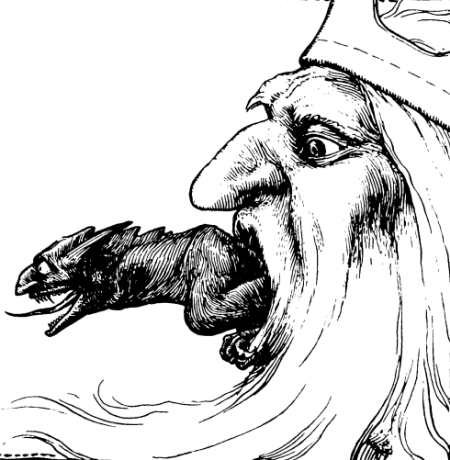
\includegraphics[scale=.35]{arcana/Tongue}
\end{wrapfigure}

Ensorcel one creature whose \HD is less than or equal to \DICE. You must touch the target's flesh (like with a handshake) when you speak the final word of this Secret. A successful \SAVE{Hexes} negates the effect; otherwise, they are \mylink{Charmed}{effect-charmed} and will regard you as a good friend and ignore the obvious enchantment you just cast on them.  The effect lasts for the entire Session unless you ask them to do something they might think was a little weird: attack an ally, let you through an area they're supposed to be guarding, etc. (this is up to the Arbiter's discretion).  This will prompt a
\RB your \INT vs. their \FOC with a -\DICE penalty. You can only have one creature Charmed at a time. The Charm can be broken and dispelled by another Charm if a Wizard Fight! is lost. 


\newpage

\WIZARDRY[
  Name=Color Spray,
  Link=secrets-color-spray,
  Alignment=Mind,
  Save=Y (negate),
  Duration=\DICE,
  Counter=None ,
  Keywords=Splittable,
  Target=Close or Nearby Monster(s)
]



You emit \DICE sprays of color from your fingertips that you can split among \DICE Monsters.  For each Monster, if the \SUMDICE of the \DICE targeting the Monster is twice as much (equal to or greater) as the Monster's \HD, it
is \mylink{Befuddled}{effect-befuddled} for the \Duration.  If \SUMDICE is three times the Monster's \HD, it is \mylink{Stunned}{effect-stunned} for a Moment, then \mylink{Befuddled}{effect-befuddled} as above. If \SUMDICE is five times the creature's \HD, it is \mylink{Stunned}{effect-stunned} for the Duration, then \mylink{Befuddled}{effect-befuddled} as above (reset the Duration die).  Save negates.





\WIZARDRY[
  Name=Commanding Presence,
  Link=secrets-commanding-presence,
  Alignment=Mind,
  Save=N,
  Duration=Combat or \SUMDICE real-world minutes,
  Counter=\mylink{Balthazar's Breathtaking Blast}{secrets-balthazars-breathtaking-blast} ,
  Keywords=None,
  Target=Self
]

You grow +\DICE meters in height, and your features and voice become terrible and commanding.  Creatures of less than \DICE \HD must test morale or flee in terror. For the duration of the Secret, you can use your \INT in place of any rolls where you would normally use \VIG.  If you enter the radius of Balthazar's Breathtaking Blast, or if the Secret is spoken Close to you, the Commanding Presence is dispelled if a Wizard Fight! is lost.




\WIZARDRY[
  Name=Ego Weapon,
  Link=secrets-ego-weapon,
  Alignment=Mind,
  Save=N,
  Duration=Session,
  Counter=\mylink{Greaseball}{secrets-greaseball} ,
  Keywords=None,
  Target=Self
]

You can summon a Bashing, Chopping, or Stabbing weapon of Force.  You can change the type of weapon by using 1 Action in Combat.  The weapon does \DICE damage and can hit creatures only affected by magic.  Only you can fight with the Ego Weapon.   You must make a successful Attack using your \INT (instead of \VIG or \DEX) to hit with the weapon.  A \mylink{Helping Hand}{secrets-helping-hand} can wield an Ego Weapon, but you can only have 1 Ego Weapon in existence at a time.  The weapon lasts for the entire Session.  It can be dispelled by a Greaseball if a Wizard Fight! is lost.

\WIZARDRY[
  Name=Enervate,
  Link=secrets-enervate,
  Alignment=Entropy,
  Save=Y (half),
  Duration=0,
  Counter=None ,
  Keywords=None,
  Target=Close or Nearby Magical Monster
]

On creatures that do not possess Blood or \mylink{Spell Dice}{monster-spell-dice}, this Secret has no effect.  Otherwise, the target of the Secret immediately takes \DICE damage for each unspent Blood/Spell Die they possess.

If 3 or more Blood Dice are spent on this Secret, the target must also immediately Save. Failure means they must immediately try \mybold{all} unspent Blood or Spell Dice as if they were manifesting them (any rolls of a 1 or a 2 loses the die; if you roll triples a Mishap occurs; etc.), though no magic will manifest.



\WIZARDRY[
  Name=Fireball,
  Link=secrets-fireball,
  Alignment=Elements,
  Save=Y (half),
  Duration=0,
  Counter=None ,
  Keywords=None,
  Target=Any point
]

You throw a ball of fire somewhere Close, Nearby, or Far Away.  Everyone Close to the detonation takes \SUMDICE+\DICE fire damage (Save for half), and highly flammable things are set aflame (curtains, dry trees, and oil but not people or buildings).




\WIZARDRY[
  Name=Fogbank,
  Link=secrets-fogbank,
  Alignment=Elements,
  Save=N,
  Duration=Concentration,
  Counter=\mylink{Mighty Lungs}{secrets-mighty-lungs} ,
  Keywords=None,
  Target=Close
]



You summon a bank of swirling and shifting fog that exists for as long as you Concentrate.  The fog can move with you, or you can take 2 Actions to mentally direct it somewhere Nearby.  The fog will blanket \SUMDICE creatures or a space \DICE+\DICE meters cubed.  Missiles that are thrown or shot into the fog strike a random target; nothing can be thrown or shot out of the fog.  The fog extinguishes small flames (torches, candles, etc). Monsters and Allies who attempt to fight while inside of the fog act as if they were \mylink{Befuddled}{effect-befuddled}.


\newpage


\WIZARDRY[
  Name=Fool's Fire,
  Link=secrets-fools-fire,
  Alignment=Entropy,
  Save=Y (negate),
  Duration=Concentration,
  Counter=\mylink{Enervate}{secrets-enervate} ,
  Keywords=Splittable,
  Target=Close or Nearby point
]

You project \DICE will-o'the-wisps into an area Close or Nearby.  The wisps can move one range (Close to Nearby, Nearby to Far Away, etc) in 1 Action.  You can split the wisps up any way you like but they can't be more than Far-Away from you.  The wisps do not shed heat, do not require air, and can't be doused by water.  They shed a steady yellow light the brightness of a torch.  At the top of the Moment, you can command up to \DICE wisps to \mylink{Befuddle}{effect-befuddled} up to \DICE Monsters that are Close to them.   Monsters get an initial Save and, if they succeed, the wisp targeting them is dispelled; otherwise, the Befuddlement lasts as long as you Concentrate. If any of the wisps are struck by an Enervate spell, they are all dispelled if a Wizard Fight! is lost.  When a wisp is dispelled, any Monsters \mylink{Befuddled}{effect-befuddled} by the wisp are released from the effect.

\WIZARDRY[
  Name=Greaseball,
  Link=secrets-greaseball,
  Alignment=Entropy,
  Save=N,
  Duration=\DICE,
  Counter=\mylink{Pritchard's Gusty Belch}{secrets-pritchards-gusty-belch} (acid) ,
  Keywords=None,
  Target=Close or Nearby Monster or Object
]

Toss a small ball of grease at a point on the ground Close or Nearby. If you would prefer to throw the ball at a person or object, make an Attack \RO using your \INT - if you miss, it dissipates.  If thrown at the ground, the surface becomes slick with a thick oil; anyone attempting to move through the area must \ROTRY{\DEX \PLUS \MD} with a -\DICE penalty, or immediately fall \mylink{Prone}{effect-prone}.  It requires a successful \RO as above to get up again.  

If you throw the Greaseball at a Monster, the effect is as above -  plus they can't hold anything without dropping it.  If you throw it at an object, the object becomes impossible to carry or hold until the grease is removed with an \mylink{Acid}{malignants-acids} (any strength), or is burned off. Pritchard's Gusty Belch (acid variety) will also dispel the grease if a Wizard Fight! is lost.  The grease is highly flammable. 

\newpage

\WIZARDRY[
  Name=Grimm's Electric Fingers,
  Link=secrets-grimms-electric-fingers,
  Alignment=Elements,
  Save=Y (half),
  Duration=0,
  Counter=None ,
  Keywords=None,
  Target=Close or Nearby Monster or Object
]

Forks of lightning erupt from your outstretched hands, striking a Close or Nearby target for \SUMDICE damage (Save for half). You can cause the
lightning to "jump" up to \DICE-1 times to another creature or object Close by, provided they are conductive (iron armor, metal ladders, etc).  Magic
swords aren't conductive.  You can "ping-pong" between two objects if you desire. Creatures struck by any bolt after the first take \DICE damage
(no Save). Objects struck by subordinate bolts will become momentarily electrified, and deal a shock that could cause someone to lose their grip unless they \RS using either their \VIG or \FOC.



\WIZARDRY[
  Name=Hammerspace Mule,
  Link=secrets-hammerspace-mule,
  Alignment=Force,
  Save=N,
  Duration=Session,
  Counter=\mylink{Illusion}{secrets-illusion} ,
  Keywords=Hammerspace,
  Target=Close
]

You create a spectral mule out of pure Force. The mule carries two \mylink{Hammerspace}{meta-hammerspace} saddlebags that can each hold \SUMDICE Burden whose combined weight doesn't exceed \DICE x 200kg (a reminder that a person is 25 Burden, and small creatures are 15).  The mule walks at a brisk trot.  It will stop and turn at your verbal command, but you cannot make it reverse or slow down. You can only give it the commands "go", "stop", "left", and "right". If the mule takes any damage, it immediately disappears and drops all the items on the ground.  The mule will obey your last command until the spell's duration expires.  Hammerspace Mules think that Illusions are real; if the Illusion would damage them in some way (a pit they would fall into, a spear they would run into, etc) the Mule is dispelled (dropping its items on the ground) if a Wizard Fight! is lost.


\WIZARDRY[
  Name=Helping Hand,
  Link=secrets-helping-hand,
  Alignment=Biomancy,
  Save=N,
  Duration=Concentration,
  Counter=\mylink{Web}{secrets-web} ,
  Keywords=None,
  Target=Self
]



You can detach either hand from its wrist.  The hand floats at chest height and can hold anything you could normally hold.  The hand can't use any weapons except for an \mylink{Ego Weapon}{secrets-ego-weapon}.  It can grab shirts, press buttons, and shove people (but not too hard).  If anyone attacks the hand, you have to roll your Guard as if they were attacking you. 
 
If your hand takes any damage, or moves further than Nearby from you, it disappears for the rest of the Session. The Hand disappears if a Wizard Fight! is lost.

\WIZARDRY[
  Name=Heroic Leap,
  Link=secrets-heroic-leap,
  Alignment=Biomancy,
  Save=N,
  Duration=0,
  Counter=None ,
  Keywords=None,
  Target=Self or Close Ally
]

You and up to \DICE-1 allies can leap +\SUMDICE meters high and/or +\SUMDICE meters forward in a straight line (in addition to distance you could normally jump).  You take no damage on landing, provided you land on or above the level you started from. For example, you could leap from the ground to top of a steeple, or you could leap over the steeple to land on the ground, but you couldn't leap from the top of a steeple to the ground.  When you land, you can make a \RSTRY{\DEX} (\RSTRY{\INT} if you are the caster) and if you succeed, you can leap again. You can do this up to \DICE times.  You can't take any Combat Actions while you're jumping around.

\WIZARDRY[
  Name=Hollow Head,
  Link=secrets-hollow-head,
  Alignment=Biomancy,
  Save=N,
  Duration=Session,
  Counter=None ,
  Keywords=Hammerspace,
  Target=Self
]


\begin{wrapfigure}[13]{r}{0.35\textwidth}
    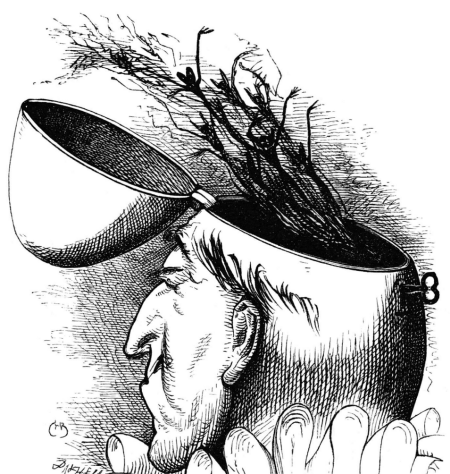
\includegraphics[scale=.35]{arcana/HollowHead}
\end{wrapfigure}


    Your brain disappears and your head has a hinge that opens like a box, but only you know this and only you can open it. For the rest of the Session,
    you are immune to the next \DICE Secrets of the Mind targeting you,  and you can fit up to \SUMDICE Burden inside of your head in \mylink{Hammerspace}{meta-hammerspace} (pulling one of these items out takes 1 Action).  When you resist the final Secret, the enchantment immediately ends. If the Secret ends while items are stored in your head, they will mix with your brain-matter. Usually this is fatal, though some Philosophers pack their head with \mylink{Narcotics}{gear-narcotics} and have a buddy speak a \mylink{Charm}{secrets-charm} Secret to them. While your head is hollow, another Philosopher could read any of the Secrets inscribed inside, just like your head was a Grimoire.

\newpage

\WIZARDRY[
  Name=Ice Bridge Step,
  Link=secrets-ice-bridge-step,
  Alignment=Elements,
  Save=N,
  Duration=Session,
  Counter=\mylink{Greaseball}{secrets-greaseball} ,
  Keywords=None,
  Target=Self
]

You and up to \DICE-1 allies can run over liquids as if they were land.  Ice forms beneath your feet with each step. If you slow down (to walk, fight,
etc), you'll sink. Very wavy seas may require you to \RSTRY{\DEX}.  Very hot liquids (like lava) may require you to \RSTRY{\INT}.  The ability is dispelled if you are struck by a Secret: Greaseball and you fail a Wizard Fight!.

\WIZARDRY[
  Name=Icebolt,
  Link=secrets-icebolt,
  Alignment=Elements,
  Save=Y (half),
  Duration=\DICE,
  Counter=None ,
  Keywords=None,
  Target=Close or Nearby point (straight line)
]

Throw a bolt of ice at a target Close or Nearby.  The bolt will travel in a straight line from your fingers.  Anything touched by the bolt takes
\SUMDICE damage, Save for half.  Additionally, everything that fails its Save is frozen to whatever surfaces they are touching.  Keys are frozen in
locks; swords are frozen to hands; boots are frozen to the ground (creatures are usually immobilized from the boots down unless they were
playing in a fountain or something).  The objects are stuck for the \Duration.

\WIZARDRY[
  Name=Illusion,
  Link=secrets-illusion,
  Alignment=Mind,
  Save=N,
  Duration=Varies,
  Counter=\mylink{Ego Weapon}{secrets-ego-weapon} ,
  Keywords=None,
  Target=Varies
]

You create an illusion of anything you desire. If anything touches the illusion, it will pass through it with no effect.  Think of the illusion as a perfectly accurate hologram that you are creating - the illusion can be
heard in addition to being seen, can perform the same action over and over again, and can deliver messages, but it can't interact in a meaningful way
or perform complex actions based on external forces. Each aspect of the illusion requires one or more Blood die to cast:

\callout{\footnotesize{

\mybullet {
  \item Having the illusion speak or make noise requires 1 \DICE for each word or sound (wailing, shouting, etc);
  \item Having the illusion appear to be a physical thing a (hole in the ground, a stone wall, orc guard, etc.) requires 1 \DICE for each square meter in size; 
  \item Having the illusion appear to move requires 1 \DICE for every meter;
  \item Having the illusion appear on a living creature (disguising them as a beggar or a lamp post) requires 1 \DICE, and they cannot be wearing or carrying any iron.
}}}

Note that there is some Arbiter's discretion here.  A guard pacing in front of a door might require 4 \DICE (a 2m tall "thing" pacing back and forth 2 meters), but more if you want them to appear more "natural" and not like a robot marching back and forth.  A disguise placed on someone to appear to be a beggar might cost 1 \DICE, but disguising yourself as the king will be significantly harder.

The Illusion will last for \DICE real-world hours.  Anyone touching the illusion will immediately know it to be fake, but this doesn't cause the illusion to disappear.  However, if the illusion is touched with an Ego Weapon, it will disappear if a Wizard Fight! is lost.


\WIZARDRY[
  Name=Invisibility,
  Link=secrets-invisibility,
  Alignment=Entropy,
  Save=N,
  Duration=\DICE,
  Counter=\mylink{Fool's Fire}{secrets-fools-fire} ,
  Keywords=None,
  Target=Self or Close Allies or Objects
]

Up to \DICE objects or creatures can be made \mylink{Invisible}{effect-invisible} (including yourself), and will remain that way as long as they don't move.  As soon as the creature or object moves (or is moved), the charm is broken.  Invisible creatures can see other invisible and hidden objects (including Knaves using Whispers).  

If this Secret is placed on something Invisible, it will force the object to become seen.  The duration of depends on the dice invested.  1 die: \SUMDICE Moments; 2 \DICE Minutes; 3 \DICE Hours; 4 \DICE Days; 5 \DICE Weeks; 6+ \DICE Forever.  The wisps from a Fool's Fire can dispel the Invisibility if a Wizard Fight! is lost.

  \myfpimage{arcana/Invisibility}


\WIZARDRY[
  Name=Kelsier's Swarm of Irritating Vermin,
  Link=secrets-kelsiers-swarm-of-irritating-vermin,
  Alignment=Force,
  Save=N,
  Duration=Combat or \SUMDICE real-world minutes,
  Counter=\mylink{Mighty Lungs}{secrets-mighty-lungs} ,
  Keywords=None,
  Target=Nearby; Far Away
]


You summon a cloud of tiny, magical, irritating vermin to an area Nearby or Far-Away.  The vermin deal \DICE damage per Moment to every living creature Close to them. If the target is an object, the vermin will do minor cosmetic damage, such as chewing holes in paper, gnawing wood, chipping paint, and scratching glass. Anything requiring Concentration is impossible within the Swarm, and any \mylink{Zoological Monsters}{monster-trait-zoological}  within the Swarm must make a Morale check or immediately flee somewhere Far-Away (this includes mounts and beasts of burden). The vermin won't move from the spot where they are summoned, and will remain until the Secret expires.  Mighty Lungs will dispel the swarm if a Wizard Fight! is lost.



\WIZARDRY[
  Name=Knife Trick,
  Link=secrets-knife-trick,
  Alignment=Force,
  Save=N,
  Duration=Session,
  Counter=\mylink{Grimm's Electric Fingers}{secrets-grimms-electric-fingers},
  Keywords=Splittable,
  Target=Close; Nearby; Far Away
]

Up to \DICE daggers orbit your head like a halo or crown (they cannot be iron).  These daggers must be in your possession, though "dagger-like" items are OK (icicles, shards of glass, etc.) at the Arbiter's discretion. At any time during the Session, you can mentally "throw" one or more of these daggers at things that are Close, Nearby, or Far-Away with unerring accuracy.  This could be used to sever a rope or pin something to a wall (or stick into someone's chest) - but no \mylink{Gambits}{combat-deeds-gambit}, that wouldn't be fair.  Each dagger does \SUMDICE+\DICE damage i.e. if you were to throw 1 dagger at someone, it would do d6+1, two daggers 2d6+2, etc.  \mylink{Grimm's Electric Fingers}{secrets-grimms-electric-fingers} will dispel the magic and cause the daggers to fall to the ground if a Wizard Fight! is lost.


\WIZARDRY[
  Name=Knock,
  Link=secrets-knock,
  Alignment=Entropy,
  Save=N,
  Duration=0,
  Counter=\mylink{Lock}{secrets-lock} ,
  Keywords=None,
  Target=Close or Nearby Objects
]


\DICE Close or Nearby object(s) is/are opened. Doors are flung wide, locks are broken, shackles are bent open, belts come undone.  Ideas or thoughts
can be unlocked from a mind if a \RBTRY{\INT}{\INT} contest is lost (target has a -\DICE penalty). Objects locked by Secret: Lock remain locked if a  Wizard Fight! is lost.


\WIZARDRY[
  Name=Levitating Disc,
  Link=secrets-levitating-disc,
  Alignment=Force,
  Save=N,
  Duration=Concentration,
  Counter=\mylink{Suspend Objects}{secrets-suspend-objects} ,
  Keywords=None,
  Target=Close or Nearby point in space
]


You draw a circle in the air of \DICE+\DICE diameter, in any orientation. The inside of the circle is made of Force, as solid as stone. You can cause the circle to raise, lower, or hover in place.  You can only move up and down (never side-to-side).  Up to \DICE people could stand under it and be completely covered, or on it and be levitated provided they don't weigh more than \DICE x200kg.  If you lower the circle on top of someone, they take \DICE damage
per Moment. The circle moves 10 meters a minute (about 3m per Moment).  You can change the disc's orientation at any time.  If the Levitating Disc is targeted with Suspend Objects, the disc will be dispelled if a Wizard Fight! is lost.


\WIZARDRY[
  Name=Lipby Chonk's Viscous Form,
  Link=secrets-lipby-chonks-viscous-form,
  Alignment=Biomancy,
  Save=N,
  Duration=Combat or \SUMDICE real-world minutes,
  Counter=None ,
  Keywords=None,
  Target=Self
]

Your flesh becomes gelatinous. You can squeeze through gaps as small as a keyhole with a great deal of effort. You take no damage from Crushing
attacks for the duration.  The Secret only affects your flesh, not anything you're wearing or carrying.


\WIZARDRY[
  Name=Lock,
  Link=secrets-lock,
  Alignment=Mind,
  Save=Y (negate),
  Duration=\DICE,
  Counter=None ,
  Keywords=None,
  Target=Close and Nearby Objects
]

Up to \DICE non-living thing slam shut and can't be opened for the \Duration. If the object is a door, chest, or something like it, it will slam shut forcefully and loudly. This Secret can work on things that aren't portals (a sword could be locked in its scabbard). You can also use this Secret to lock a specific memory or thought, making it immune to mind reading or scrying without a \RBTRY{\INT}{\INT}.  The Lock can be dispelled by the Secret: Knock if a Wizard Fight! is lost.


\WIZARDRY[
  Name=Meat Shield,
  Link=secrets-meat-shield,
  Alignment=Biomancy,
  Save=N,
  Duration=\DICE real-world hours,
  Counter=None ,
  Keywords=None,
  Target=Close and Nearby
]

You summon a giant slab of meat that fills an area \DICE meters cubed.  The meat weighs \DICE x100kg and lasts for \DICE real-world hours. \mylink{Zoological Monsters}{monster-trait-zoological} will attack the Meat Shield first. When the Meat Shield has been dealt \SUMDICE+\DICE damage or more to the Meat, consider it consumed/destroyed. During a \mylink{Bivouac}{combat-resting-bivouac}, up to \DICE Allies can eat the Meat Shield in lieu of rolling their Provisions, but the provenance of the meat is ... unknown.  If a Scything Disc of Nog is used on a Meat Shield, the shield will be dispelled if a Wizard Fight! is lost (otherwise, it will take damage as normal).

\WIZARDRY[
  Name=Mighty Lungs,
  Link=secrets-mighty-lungs,
  Alignment=Biomancy,
  Save=N,
  Duration=Until exhalation,
  Counter=None ,
  Keywords=Contested,
  Target=Self
]

Your next inhalation allows you inhale 10x the normal amount of air. Not only does this allow you to hold your breath for 10x as long, but if you
exhale forcefully it will release a blast of air strong enough to knock pigeons out of air and polish your teeth. A human-sized creature is knocked
\mylink{Prone}{effect-prone} and pushed Nearby unless they try a \RB \DEX or \VIG (their choice) with a -\DICE penalty vs your \INT.  This Secret will also blow open all closed but unlocked doors in a room, shatter all windows in a building, or knock the thatched roof off a peasant's shack.

\WIZARDRY[
  Name=Mirror Image,
  Link=secrets-mirror-image,
  Alignment=Entropy,
  Save=N,
  Duration=Session,
  Counter=None ,
  Keywords=None,
  Target=Self
]

You create \DICE illusory images of yourself, which move as you move and always stay Close to you. They are constantly stepping through each other,
making it impossible to determine which representation of you is "real". When an enemy attacks you, they'll always hit an image first.  An image vanishes as soon as it suffers
a solid impact (a blow from a mace, but also a slap). Area effects such as a dragon's breath will cause all images to instantly vanish (and you take the
damage, naturally). Finally, invoking \mylink{Mirror Image}{secrets-mirror-image} causes any other images that already exist to immediately vanish.


\WIZARDRY[
  Name=Morass,
  Link=secrets-morass,
  Alignment=Elements,
  Save=N,
  Duration=Concentration,
  Counter=\mylink{Bastogne's Glamping Charm}{secrets-bastognes-glamping-charm} ,
  Keywords=Contested,
  Target=Nearby or Far-Away Area
]

The ground \SUMDICE meters in radius and \DICE meters deep turns to black muck.  Monsters and objects in the mud sink 1 meter per Moment.  At the top of
the Moment, a creature can \RB: \VIG with a -\DICE penalty vs. your \INT to pull themselves out 1 meter (if they were only 1 meter deep to begin with, they escape).  If someone's head dips below the mud (2m for people, 1m for Pooka, 4m or more for giants), they immediately being drowning and must make a \DEATH roll at the top of every Moment they are submerged (they can still claw their way up 1m with a successful \RB try, as above).  If they don't have a \DEATH, they die in \HD Moments.

The Secret lasts for as long as you \mylink{Concentrate}{time-concentration}.  When you break your Concentration, everything that sunk in the mud is immediately vomited back to the surface. If the area covered by the Morass is targeted by Bastogne's Glamping Charm, the Morass will be dispelled (and the objects brought to the surface) if a Wizard Fight! is lost.


\WIZARDRY[
  Name=Negasonic Bomb,
  Link=secrets-negasonic-bomb,
  Alignment=Mind,
  Save=N,
  Duration=Concentration,
  Counter=\mylink{Cacophony}{secrets-cacophony} ,
  Keywords=None,
  Target=Nearby or Far Away Area
]

You roll a small orb of Mind to a point Close, Nearby or Far-Away; the orb rolls silently and is hard to see.  When the orb stops rolling it immediately and silently detonates.  Creatures Close to the designated point are \mylink{Deafened}{effect-deafened} until they move somewhere Nearby; likewise, no sound can be made (including speaking) while Close to the point of detonation. Arcana and skills that require vocalization are impossible within this area of silence, which lasts as long as you \mylink{Concentrate}{time-concentration}.  The bomb can be dispelled by Cacophony if a Wizard Fight! is lost.



\WIZARDRY[
  Name=Prismatic Ray,
  Link=secrets-prismatic-ray,
  Alignment=Entropy,
  Save=Y (half),
  Duration=0,
  Counter=None ,
  Keywords=Splittable,
  Target=Nearby or Far-Away
]

A brilliant white light emanates from your forehead to a point Nearby or Far-Away, where it splits into a prism of \DICE beams.  Each beam strikes a
random Monster Close to the prism (roll for each beam; a Monster can be hit by more than 1 beam).  Roll a d8 on the table below for each beam and apply its results.

\callout{\footnotesize{

\mynumlist {
  \item \mybold{Red} Target takes \DICE fire damage, Save for half. Highly flammable things catch fire.
  \item \mybold{Orange}  Target takes \DICE bashing damage, Save for half. 
  \item \mybold{Yellow} Target takes \DICE lightning damage, Save for half.  If you fail your Save, you drop what you're holding.
  \item \mybold{Green} Target takes \DICE acid damage, Save for half. Roll your Armor \UD if applicable.
  \item \mybold{Blue} Target takes \DICE ice damage, Save for half. If you fail your Save, you fall \mylink{Prone}{effect-prone}.
  \item \mybold{Indigo} Target takes \DICE stabbing damage, Save for half.
  \item \mybold{Violet} Target takes \DICE chopping damage, Save for half.
  \item \mybold{Roll} again.  Instead of \DICE damage, the effect deals \SUMDICE damage.. If you get this result again, the beam splits and the target takes an additional effect (roll again and apply the result).  Continue in this way until you don't roll an 8.
}}}


\WIZARDRY[
  Name=Pritchard's Gusty Belch,
  Link=secrets-pritchards-gusty-belch,
  Alignment=Biomancy,
  Save=N,
  Duration=0,
  Counter=None ,
  Keywords=None,
  Target=Close and Nearby Area
]

You can breathe out up to \DICE elements (fire, acid, water, wind, steam, etc) immediately in front of you for a Moment.  The elements don't interact with one another and act independently, so if you were to belch out fire and water, you would get the effects of both.  If the order matters (set something on fire and immediately douse it with water), you pick the order of effects.  Water breath is enough to extinguish fires smaller than a big bonfire, or wash off acid; wind breath could push a small sailboat or blow swarming insects out of an area; acid breath bleaches the color from objects and irritates the eyes; fire breath would cause paper and flammable objects (but not people, unless they were doused in oil) to catch fire, etc.


\WIZARDRY[
  Name=Protection from Element,
  Link=secrets-protection-from-element,
  Alignment=Elements,
  Save=N,
  Duration=Session,
  Counter=\mylink{Prismatic Ray}{secrets-prismatic-ray} ,
  Keywords=Splittable,
  Target=Self or Close Allies
]

Reduce all damage of a single chosen element (acid, cold, fire, lightning, etc) by -\DICE per die (minimum of 1).  The Secret protects its targets from the negative effects of the natural elements (desert heat, arctic chill) as well.  If you are struck by a Prismatic Ray of the same elemental type, the protection is dispelled if a Wizard Fight! is lost.

\myfpimage{arcana/Wizardry_1}



\WIZARDRY[
  Name=Rhea's Efficacious Plow,
  Link=secrets-rheas-efficacious-plow,
  Alignment=Force,
  Save=N,
  Duration=Moments,
  Counter=None ,
  Keywords=None,
  Target=See description
]

You send an invisible wedge of Force along the ground in a straight line up to a Distant point. The wedge can take up to \DICE left or right turns at your command. Any light debris in the path (snow, small stones, leaves, grass) is pushed to the side; fields can be tilled. Any pressure plates or tripwires are activated. You do not have to be able to see the entire path, but you do need to know the approximate route the wedge will take. The wedge can't move through solid objects, and it can't directly hurt anyone (though it will push them to the side). The path cleared is \DICE meters wide. If you cast this Secret with 3+ \DICE, the width becomes \SUMDICE meters wide.

\WIZARDRY[
  Name=Sandstorm,
  Link=secrets-sandstorm,
  Alignment=Elements,
  Save=N,
  Duration=Concentration,
  Counter=None ,
  Keywords=None,
  Target=Close
]

You cough up a swirling spiral of sand.  Small flying creatures (bug-sized) and missile weapons cannot enter or leave the sandstorm.  Up to \DICE-1 other
people can hide in the sandstorm with you.  The sand moves with you and lasts as long as you \mylink{Concentrate}{time-concentration}.



\WIZARDRY[
  Name=Sanguine Mail,
  Link=secrets-sanguine-mail,
  Alignment=Biomancy,
  Save=N,
  Duration=Session or until Exhausted,
  Counter=\mylink{Enervate}{secrets-enervate} ,
  Keywords=None,
  Target=Self
]


You become encased in elaborate plate mail that seems to be made from constantly congealing blood.  You definitely stand out in a crowd. Your \MD drops to d8.  The \UD for the Armor depends on the number of \DICE invested: 1 d4; 2 d8; 3+ d12. You can only have one Sanguine Mail active at a time. If you are struck with an Enervate spell, the Sanguine Mail is dispelled if a Wizard Fight! is lost.


\WIZARDRY[
  Name=Scuttle,
  Link=secrets-scuttle,
  Alignment=Biomancy,
  Save=N,
  Duration=Combat or \SUMDICE real-world minutes,
  Counter=\mylink{Greaseball}{secrets-greaseball} ,
  Keywords=None,
  Target=Self
]


Your clothes and hair animate to carry you around. You can move at full speed in any orientation, and you can freely rotate as you move. For
instance, you could run while standing on your head, holding a torch, and turning counterclockwise. You can lie on your side and, while flipping end
over end, move backwards. This effect does not allow you to climb up walls, but ladders and ropes are no problem (you could suspend yourself from a rope
and cast spells, for example).  If you are struck with a Greaseball, or attempt to climb something affected by Greaseball, the Scuttle is dispelled if a Wizard Fight! is lost.




\WIZARDRY[
  Name=Scything Disc of Nog,
  Link=secrets-scything-disc-of-nog,
  Alignment=Force,
  Save=Y (half),
  Duration=0,
  Counter=None ,
  Keywords=None,
  Target=Nearby or Far Away Area
]

You hurl a whirling disc of Force and light from your fingertip. The disc screeches like a sawblade. It deals \SUMDICE damage to its target, Save for
half. If it deals more than 6 damage, it bounces towards a random creature (friend, foe, or even yourself) Close or Nearby, dealing \SUMDICE-2
damage, Save for half. If it deals more than 6 damage, it bounces towards another random creature Close or Nearby, dealing \SUMDICE-4 damage, Save for
half. This continues, losing 2 damage with each bounce, until there are no valid targets or the Secret deals 6 or less damage to a creature.


\WIZARDRY[
  Name=Sleep,
  Link=secrets-sleep,
  Alignment=Mind,
  Save=Y (negate),
  Duration=\DICE,
  Counter=\mylink{Cacophony}{secrets-cacophony} ,
  Keywords=None,
  Target=Close or Nearby Area
]

You summon a cloud of somnolent dust to a point Close or Nearby. \SUMDICE creatures Close to the cloud, who have no more than \DICE \mylink{Hit Dice}{monster-hit-dice}, must
immediately Save or fall into a magical slumber.   They can't be awakened by anything less than a vigorous slap (counts as 1 Action).  You don't have
control over who falls asleep, it's entirely random - but will be as many creatures as possible (up to \SUMDICE), which means lower \HD creatures will go to sleep first.  You are immune to your own Secret: Sleep (so you could cast it Close to yourself).  Creatures who fall asleep immediately fall \mylink{Prone}{effect-prone} and drop any items they're holding.  Attack tries against them will hit automatically and do maximum damage, and can only be blocked by Armor.  This will wake the creature up, of course.  If an orb of Cacophony is detonated Nearby, the creatures will awaken if a Wizard Fight! is lost.  Otherwise, creatures who fall asleep will remain asleep for the \Duration.  


\WIZARDRY[
  Name=Summon Candles,
  Link=secrets-summon-candles,
  Alignment=Force,
  Save=N,
  Duration=Session or until used,
  Counter=\mylink{Fogbank}{secrets-fogbank} ,
  Keywords=None,
  Target=Close
]

\SUMDICE dribbling candles appear on objects you touch. You can walk around placing candles as required for Minutes. The candles are lit and burn for
the entire Session (though see below). They can be detached, but will fade from existence within Minutes unless reattached.  

For every 6 candles that are Nearby to you, you may do one of the following:

\callout{\footnotesize{

\mybullet {
    \item Gain a +4 on a Wizard Fight! try;
    \item Cause a physical attack that would hit you to miss instead; 
    \item \mylink{Nudge}{dice-nudge} one of your rolled Blood Dice to a natural 6;
    \item Reduce a Ruin to a Calamity; a Calamity to a Mishap; or take no effect from a Mishap
}}}

When you use any of these powers, 6 candles immediately disappear. You must have at least 6 candles Nearby to use a power (no "rounding up"). The candles disappear at the end of the Session if they're not used. Candles encased in a Fogbank are snuffed out and dispelled if a Wizard Fight! is lost.


\WIZARDRY[
  Name=Suspend Objects,
  Link=secrets-suspend-objects,
  Alignment=Force,
  Save=Y (negate),
  Duration=Concentration,
  Counter=\mylink{Levitating Disc}{secrets-levitating-disc} ,
  Keywords=None,
  Target=Any Distance
]


You can hold up to \DICE objects in the air, weighing no more than \DICE x200kg.  You can allow these objects to descend at 3m per Moment at your
discretion. Creatures who are brought to ground in this way take no damage from \mylink{Falling}{movement-falling}. Unwilling creatures (flying Monsters, for example) get a Save to negate if you attempt to force them to the ground.  If a Levitating Disc is summoned in the midst of the held creatures, the Secret: Suspend Objects will be dispelled (and the objects will fall) if a Wizard Fight! is lost.


\WIZARDRY[
  Name=Tempestuous Chariot,
  Link=secrets-tempestuous-chariot,
  Alignment=Elements,
  Save=N,
  Duration=One trip,
  Counter=None ,
  Keywords=None,
  Target=Close
]

A tumult of air elementals lifts you and \DICE-1 others and takes you in any direction you desire, up to \SUMDICE km away.   One catch - the elementals can only travel in a straight line, and you have to choose beforehand the way to go ("up", "east", "that way", etc).  While you are in the tempest you are buffeted horribly and can neither talk nor act.  The winds refuse to travel without you, and will immediately dispel if you lose contact.


\WIZARDRY[
  Name=Vertigo,
  Link=secrets-vertigo,
  Alignment=Mind,
  Save=Y (negate),
  Duration=\DICE,
  Counter=\mylink{Suspend Objects}{secrets-suspend-objects} ,
  Keywords=None,
  Target= Any Distance
]

You can cause up to \DICE Close, Nearby, Far-Away, or Distant creatures to suffer severe vertigo unless they Save.  Creatures that are climbing or
flying immediately fall; creatures who are Close to the edge of something (a cliff, a wall, the guardrails of a ship, etc) need to \RSTRY{\FOC} or fall.
Creatures already on the ground will fall \mylink{Prone}{effect-prone} for the \Duration. If the creatures are struck with a Suspend Objects spell, the Vertigo is dispelled if a Wizard Fight! is lost.

\newpage

\WIZARDRY[
  Name=Web,
  Link=secrets-web,
  Alignment=Entropy,
  Save=Y (negate),
  Duration=\DICE,
  Counter=None ,
  Keywords=None,
  Target=Nearby or Far Away Area
]

You can anchor a giant web between three or more solid points up to \DICE meters in radius (for example: the 4 points of a door, two trees and the ground, across a hallway, etc).  Objects that touch the web immediately become stuck; arrows and spears can't be fired through it.  Creatures that enter the web (or are caught in it when cast) must Save or become ensnared for \Duration (each creature must make its \Duration try separately). Attack tries against them hit automatically and can only be blocked by Armor.  The web is extremely flammable and will be consumed in \DICE Moments.

\myfpimage{arcana/Spider}

\WIZARDRY[
  Name=Whirling Blades,
  Link=secrets-whirling-blades,
  Alignment=Entropy,
  Save=N,
  Duration=Concentration,
  Counter=\mylink{Suspend Objects}{secrets-suspend-objects} ,
  Keywords=None,
  Target=Self
]

You summon a number of invisible blades of Force that spin around your waist, with you in the center.  Every creature Close to you takes \DICE+\DICE
damage for each Moment the Secret is maintained.  The blades will cut or damage fragile objects.  If the creature or object sits above or below your waist, they take no effect.  If the blades are struck by a Secret: Suspend Objects, they will be dispelled if a Wizard Fight! is lost.

\begin{multicols}{2}

    \newpage  
}%end

